\chapter{Descripción las herramientas implementadas}\label{chapter:implementation}
El objetivo de este trabajo es la informatización de los 
procesos de asignación de docencia y 
planificación de las tesis que se llevan a cabo 
en la Facultad de Matemática y Computación de la Universidad de La Habana (MATCOM). 

En este capítulo se presenta la aplicación web que se implementó 
como propuesta de solución para la informatización de estos procesos. 
En las secciones \ref{cap4:docencia} y \ref{cap4:tesis} se describen los pasos que se deben 
seguir para realizar a través del sistema, la asignación de docencia y la planificación de las tesis, respectivamente.
En la sección \ref{cap4:csv} se describe una funcionalidad que se implementó en el lado del servidor 
para salvar el estado de la base datos en documentos CSV y poblar la base de datos a partir de los mismos.

% P

% En este capítulo se presenta 

% la propuesta de solución para 
% la informatización de los procesos de asignación de docencia y 
% planificación de las tesis que se llevan a cabo 
% en la Facultad de Matemática y Computación de la Universidad de La Habana. 




% Se implementó un sistema de gestión siguiendo el modelo cliente-servidor. El desarrollo del servidor se efectuó con el uso Django, en 
% particular Django Rest Framework y el cliente se desarrolló utilizando
% Quasar para la creación de las interfaces de usarios. Para almacenar los datos que 
% se utilizó una base de datos SQLite.

En la figura \ref{img-home-page} se ilustra la vista inicial de la 
aplicación web que se implementó. En la parte superior se encuentra una 
barra de navegación, desde la cual se puede acceder a todas las vistas 
de la aplicación. Se crearon dos paneles principales, uno para la administración de 
los departamentos y otro para la planificación de las tesis. En el 
panel para la administración de los departamentos se muestran los cuatro departamentos 
de la facultad MATCOM, con cuatro botones cada uno que llevan a las vistas 
para administrar los profesores, las asignaturas, las cargas de las asignaturas 
y las asignaciones de docencia correspondientes al departamento.
En el panel para la planificación de las tesis se agregó un selector para definir qué curso escolar 
se desea planificar y tres botones que 
llevan a las vistas para administrar las tesis, los tribunales y las defensas, correspondientes 
al curso escolar seleccionado.

  


\begin{figure}[H]
    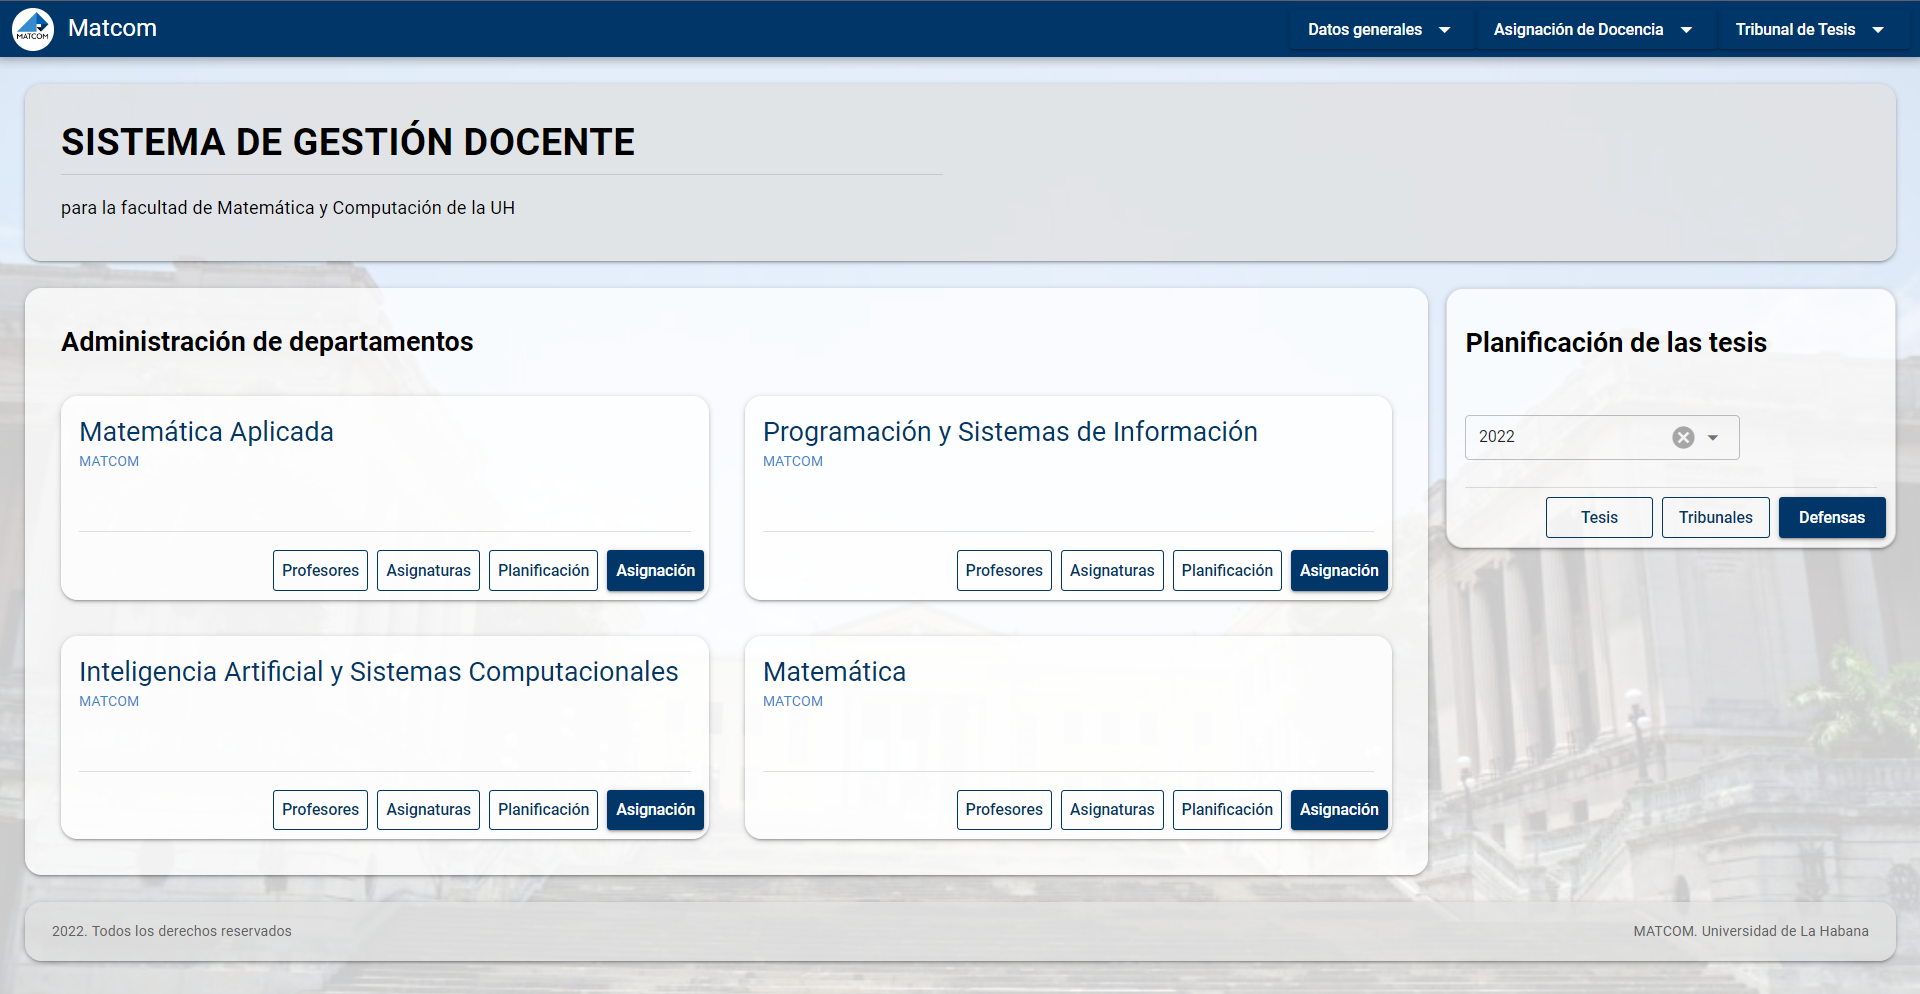
\includegraphics[scale=0.3]{Graphics/Implementation/Home-page.png}
    \caption{Vista inicial del sistema de gestión}
    \label{img-home-page}
\end{figure}






\section{Asignación de docencia}\label{cap4:docencia}

% El proceso de asignación de docencia en un departamento se realiza en la 
% interfaz que se muestra en la figura \ref{img-ta-done}. El usuario de la 
% aplicación puede ver la carga docente de los profesores durante el proceso 
% de asignación, realizar filtrados por profesor para ver las asignaturas 
% que tiene asignada y descargar un documento CSV que contiene la información 
% de la docencia una vez haya terminado la asignación.



En esta sección se describen los pasos que se deben seguir para realizar 
el proceso de asignación de docencia en un departamento a través del sistema 
de gestión que se propone en este trabajo. 
Para la ilustrar este proceso se utilizará 
el mismo fragmento de la docencia correspondiente al departamento
de Matemática Aplicada en el período de tiempo 
enero--julio del curso 2022, que se describe en la sección \ref{docencia:cap2}. 
En la tabla \ref{tabla-carga-asignaturas-cap4} 
se muestra la carga de las asignaturas que se deben impartir
y en la \ref{tabla-carga-asignaturas-cap4} 
la distribución de los profesores
para cubrir con la docencia. 
% Supongamos que se quiere realizar la asignación de docencia para el departamento 
% de Matemática Aplicada   

% \begin{table}[H]
%     \centering
%     \begin{tabular}{| c | c | c | c | c |}
%         \hline
%         \thead{Facultad}   & \thead{Año} & \thead{Asignatura} & \thead{Horas} & \thead{Grupos}  \\ \hline
%         MATCOM     & M3  & Optimización Matemática I  &  64   &  1/1   \\ 
%         MATCOM     & C3  & Modelos de Optimización I  &  64   &  1/2   \\ 
%         GEOGRAFÍA  & G2  & Estadística                &  80   &  1/2   \\ 
%         \hline
%     \end{tabular}
%     \caption{Fragmento de la planificación de docencia.}
%     \label{tabla-planificación-cap4}
% \end{table}

\begin{table}[H]
    \centering
    \begin{tabular}{| c | c | c | c | c | c |}
        \hline
        \thead{Asignatura}  & \thead{Año} & \thead{Facultad} & \thead{Horas} & \thead{Grupos} & \thead{\makecell{Distribución \\ de horas}  } \\ \hline
        Optimización Matemática I  & M3  & MATCOM  &  64   &  1/1  & 32/32  \\ 
        Modelos de Optimización I  & C3  & MATCOM  &  64   &  1/2  & 32/32  \\ 
        Estadística                & G2  & GEOGRAFÍA  &  80   &  1/2  & 48/32  \\ 
        \hline
    \end{tabular}
    \caption{Carga de las asignaturas}
    \label{tabla-carga-asignaturas-cap4}
\end{table}


\begin{table}[H]
    \centering
    \begin{tabular}{ | c | c | c | c |}
      \hline
      \thead{Asignatura} & \thead{Horas} & \thead{Grupos} & \thead{Profesores}\\
      \hline
      Optimización Matemática I &  64  & 1/1 & \makecell{C: Aymée Marrero (32) \\ CP: Gemayqzel Bouza(32)} \\
      \hline
      Modelos de Optimización I   &  64   &  1/2 & \makecell{C: Aymée Marrero(16) \\ C: Fernando Rodríguez (16) \\ CP: Daniela González(32) \\ CP: Camila Pérez(32)}    \\ 
      \hline
      Estadística                 &  80   &  1/2 &  \makecell{C: Elianys García (48) \\ CP: Ernesto Borrego(32) \\ CP: Elianys García(32)} \\  
      \hline
    \end{tabular}
    \caption{Fragmento de la asignación de docencia.}
    \label{tabla-asignación-cap4}
\end{table}


El primer paso que se debe realizar es planificar la carga de las asignaturas 
que se deben impartir, la interfaz de usuario que se implementó en el sistema para realizar 
este proceso se muestra en la figura \ref{img-pd-example}.

\begin{figure}[H]
    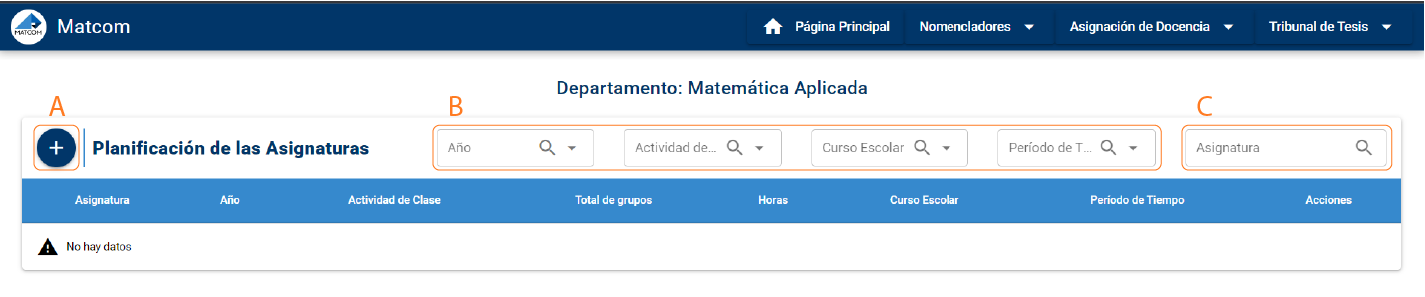
\includegraphics[scale=0.3]{Graphics/Implementation/Docencia/PD-empty.png}
    \caption{Vista de la planificación de las cargas de las asignaturas}
    \label{img-pd-example}
\end{figure}


En la figura \ref{img-pd-example},
se indican con recuadros tres regiones cuyo significado se explica a continuación.

\begin{itemize}
    \item A: botón para agregar una nueva carga de asignatura.
    \item B: filtros por: Año, Actividad de clase, Curso escolar, Período de tiempo.
    \item C: barra de búsqueda por texto para el nombre de las asignaturas. 
\end{itemize}


Para agregar una nueva carga de asignatura se debe pulsar en el 
botón que se indica en el recuadro A y completar los campos del formulario. 
En la figura \ref{img-pd-form} se muestra como agregar la planificación
correspondiente a las conferencias de la asignatura Optimización
Matemática I para los estudiantes de tercer año de la carrera Matemática. 

\begin{figure}[H]
    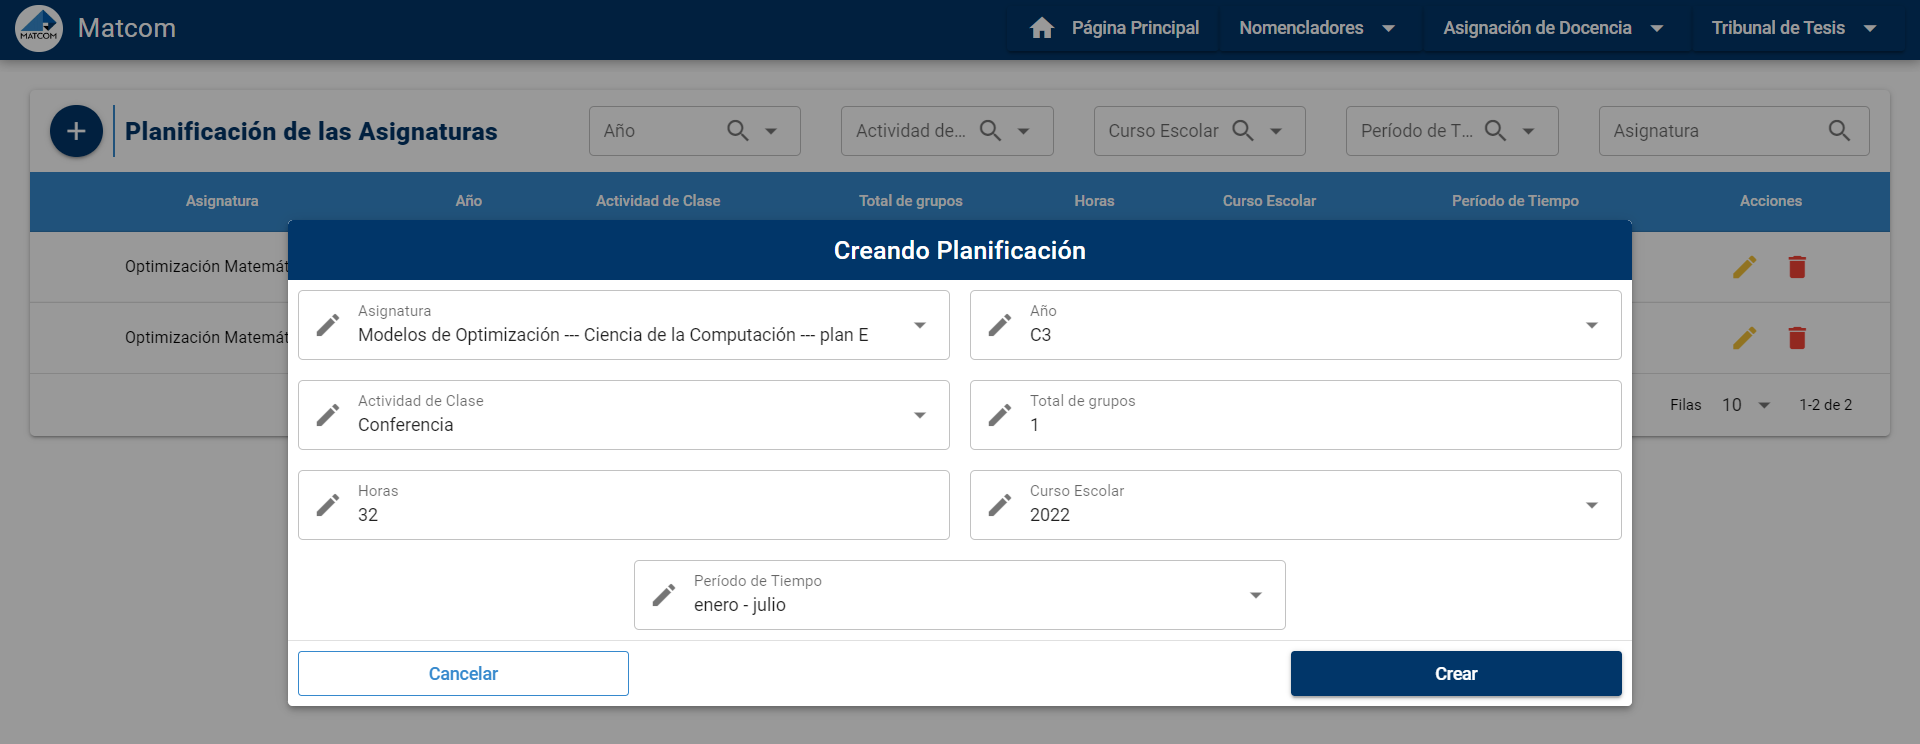
\includegraphics[scale=0.3]{Graphics/Implementation/Docencia/PD-form.png}
    \caption{Vista del formulario para crear una carga de asignaturas}
    \label{img-pd-form}
\end{figure}


La figura \ref{img-pd-result} muestra el resultado de agregar las planificaciones de las asignaturas 
correspondientes a la tabla \ref{tabla-carga-asignaturas-cap4}. 


\begin{figure}[H]
    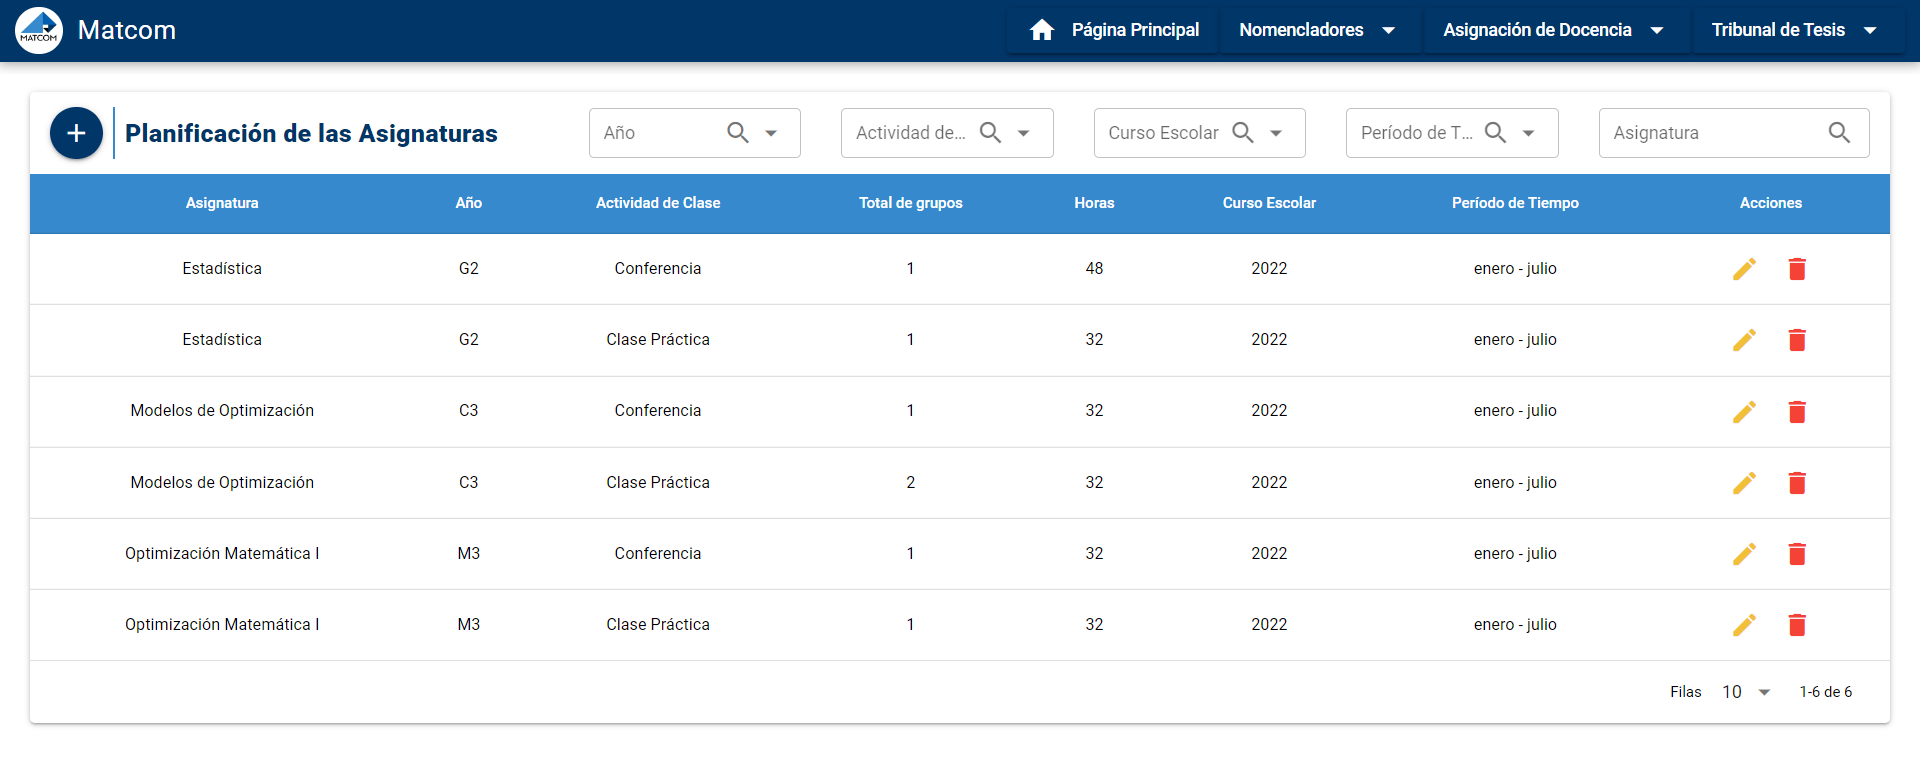
\includegraphics[scale=0.3]{Graphics/Implementation/Docencia/PD-result.png}
    \caption{Vista de la carga de las asignaturas}
    \label{img-pd-result}
\end{figure}

Por cada carga de asignatura que se agregue en el sistema se crean $n$ asignaciones 
de docencia sin asignar, donde $n$ es la cantidad de grupos que tiene la carga de la asignatura. En 
la figura \ref{img-ta-unassing} se muestran las asignaciones de docencias creadas automáticamente por el sistema 
a partir de las cargas agregadas en la figura \ref{img-pd-result}.

\begin{figure}[H]
    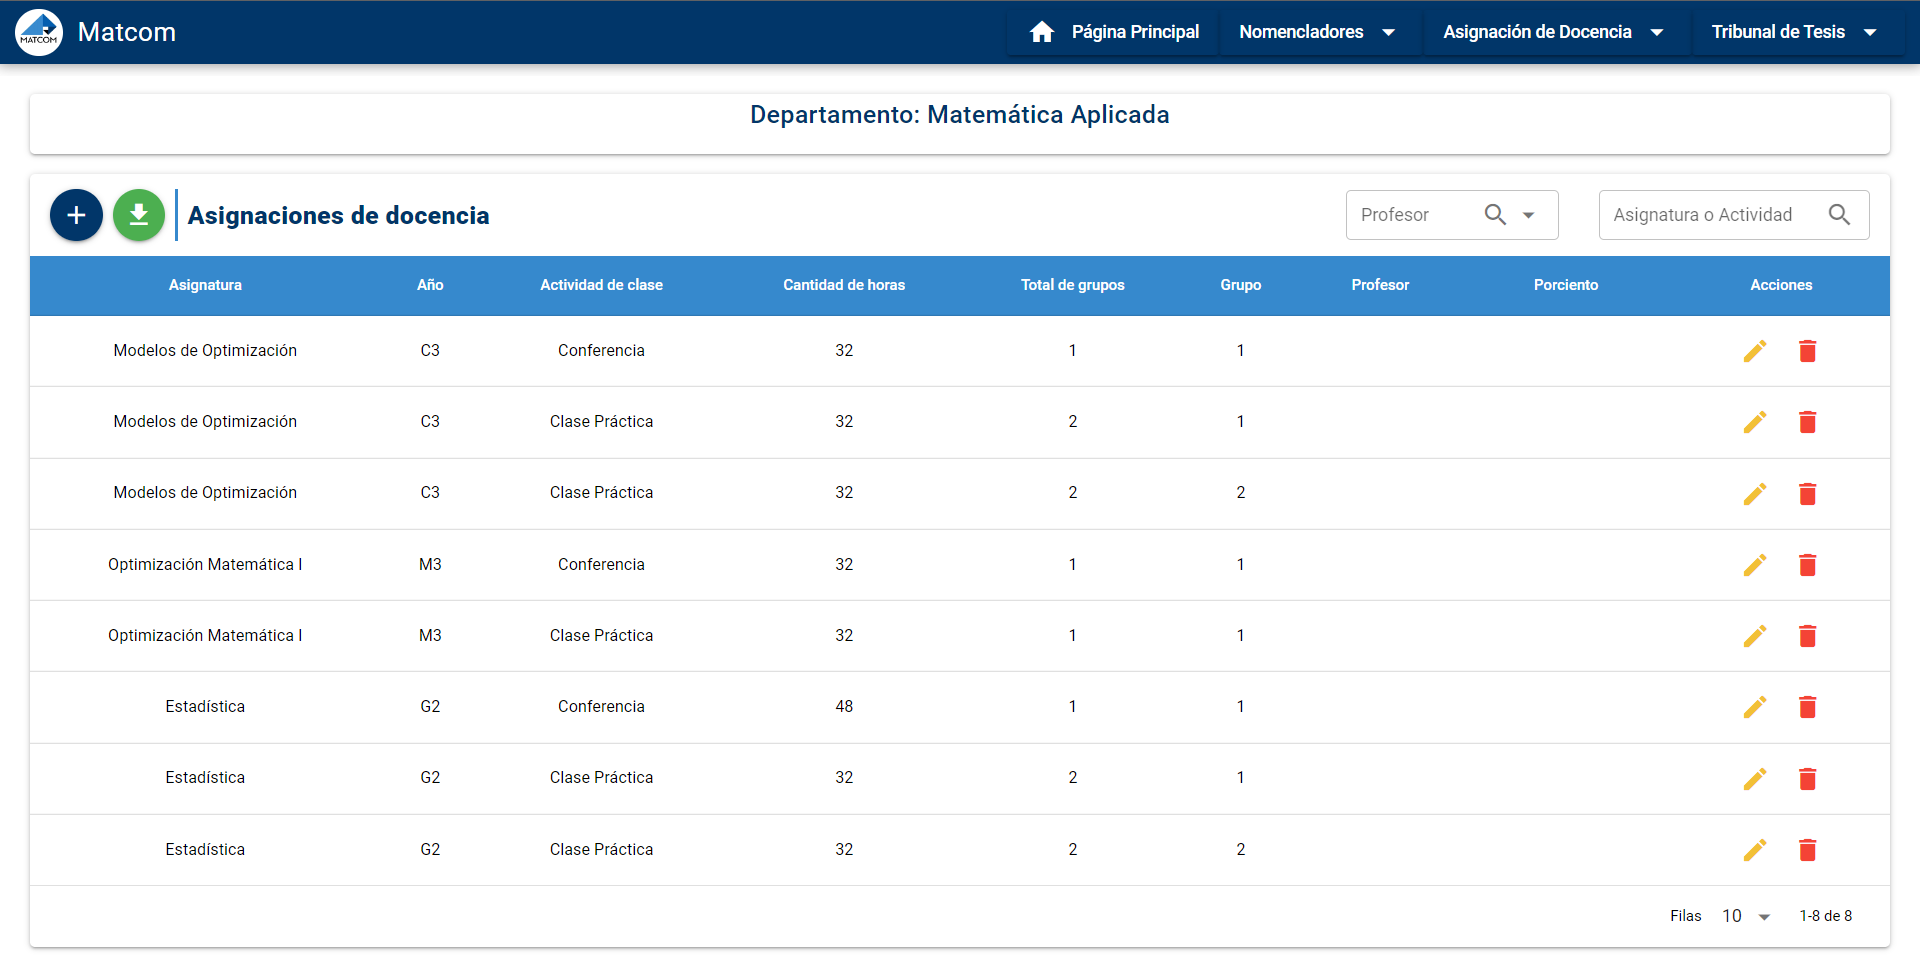
\includegraphics[scale=0.3]{Graphics/Implementation/Docencia/AD-unassing.png}
    \caption{Vista de la asignación de docencia}
    \label{img-ta-unassing}
\end{figure}


El próximo paso es realizar la asignación de los profesores para cubrir 
la docencia del semestre. Para asignar un profesor se debe 
pulsar sobre el botón de editar de una fila. En la figura \ref{img-ta-form-empty} se muestra el resultado 
de pulsar sobre el botón de editar de la cuarta fila, correspondiente a las conferencias
de la asignatura de Optimización Matemática I. 


\begin{figure}[H]
    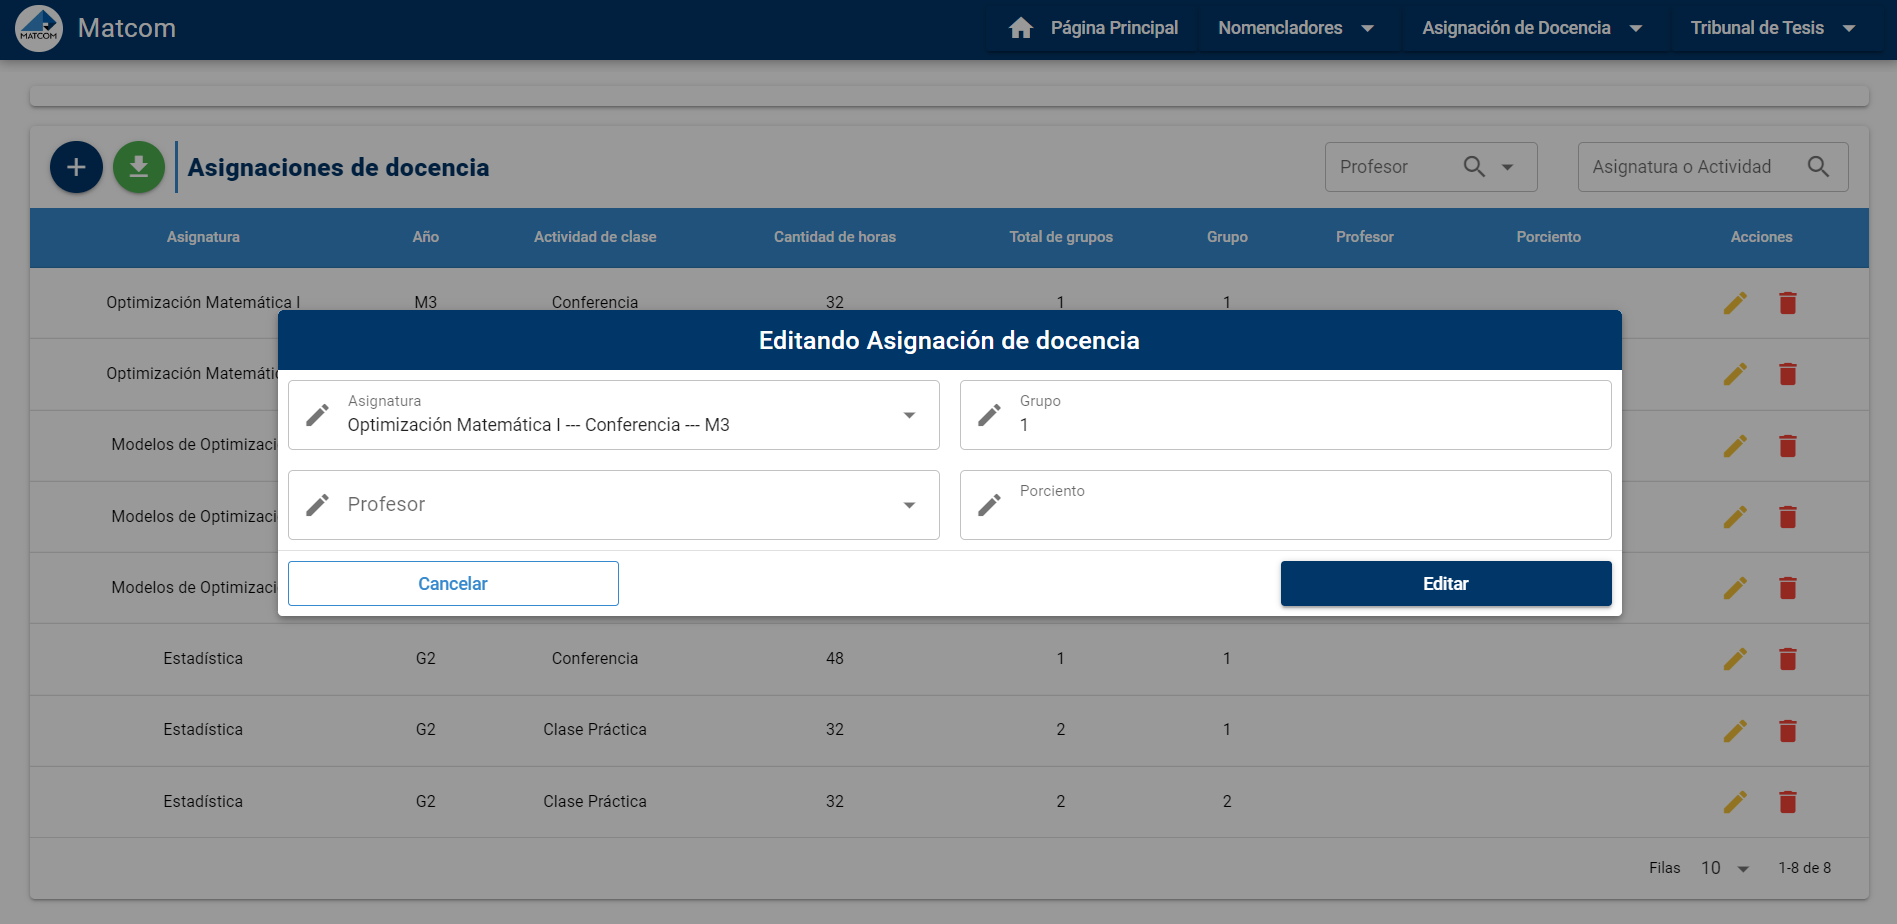
\includegraphics[scale=0.3]{Graphics/Implementation/Docencia/AD-form-empty}
    \caption{Vista del formulario para realizar una asignación de docencia}
    \label{img-ta-form-empty}
\end{figure}


Se deben completar los campos del formulario y pulsar sobre el botón editar. 
Como se muestra en la tabla \ref{tabla-asignación-cap4}, la profesora Aymée Marrero es la encargada de 
impartir las 32 horas de conferencia de la asignatura Optimización Matemática I, por 
tanto se debe especificar que la profesora imparte el 100 porciento de las horas 
como se muestra en la figura \ref{img-ta-form-fill}.


\begin{figure}[H]
    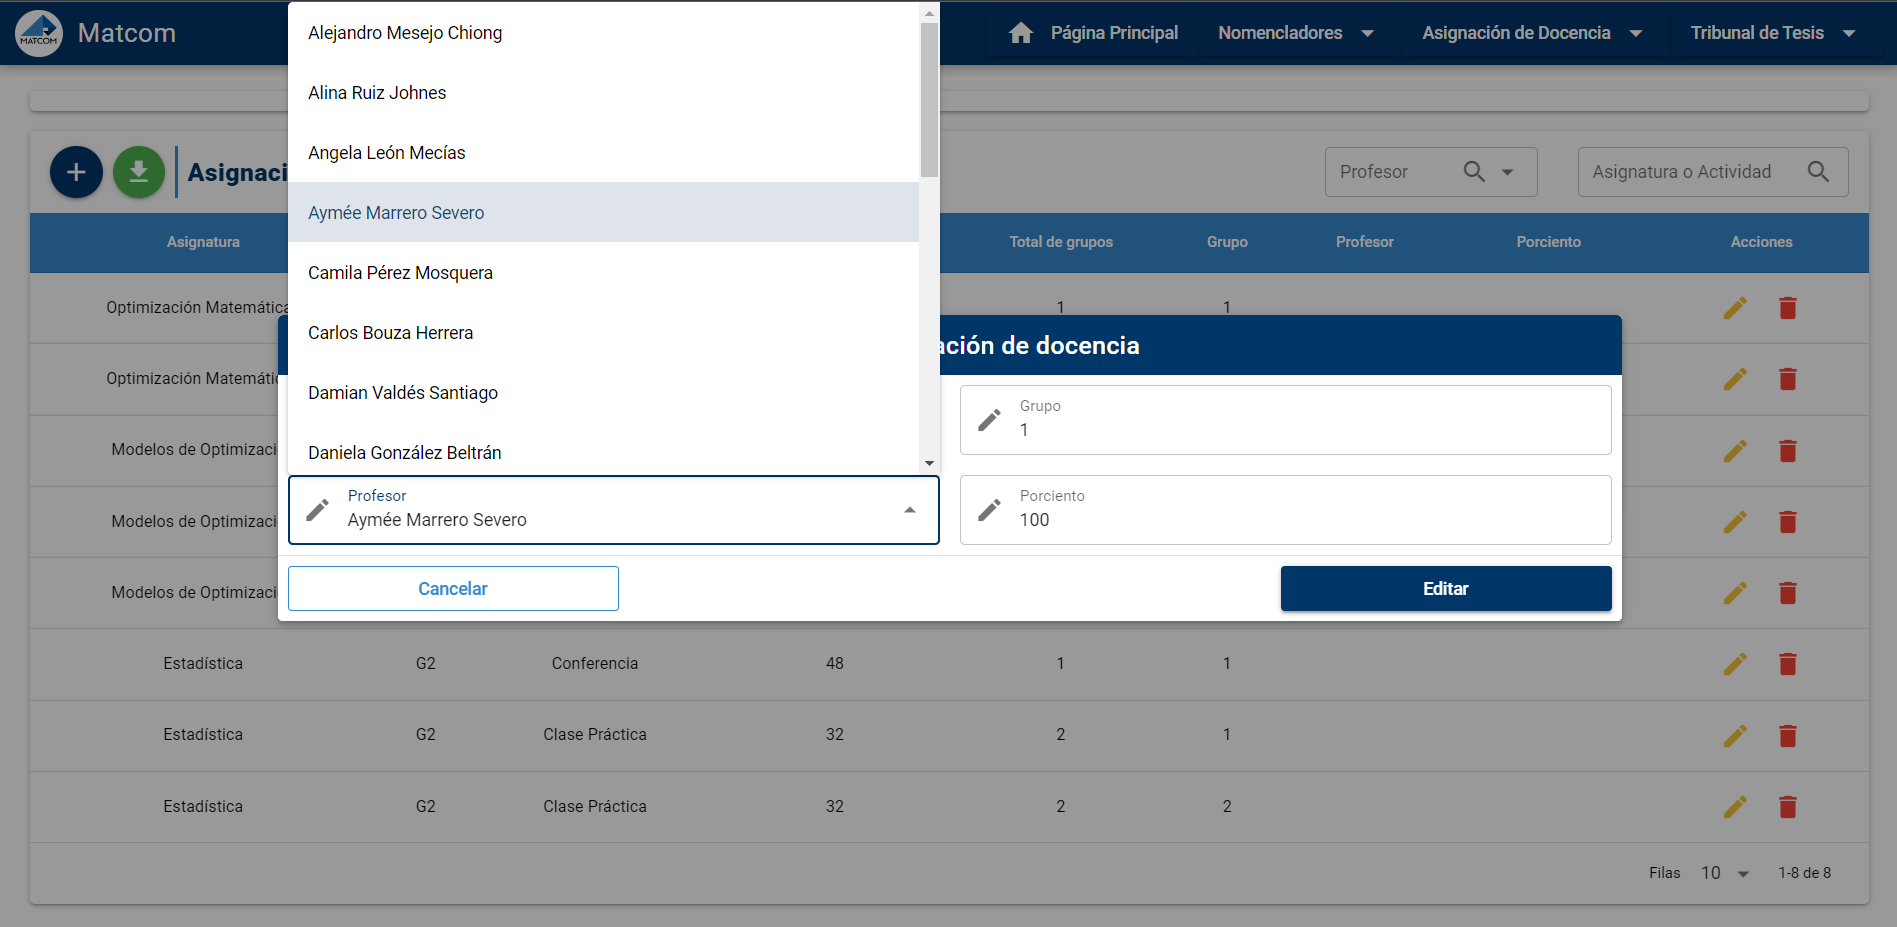
\includegraphics[scale=0.3]{Graphics/Implementation/Docencia/AD-form-fill.png}
    \caption{Vista del formulario con los datos ingresados de una asignación de docencia}
    \label{img-ta-form-fill}
\end{figure}


En la figura \ref{img-ta-one-assign} se muestra el resultado 
de realizar la asignación.


\begin{figure}[H]
    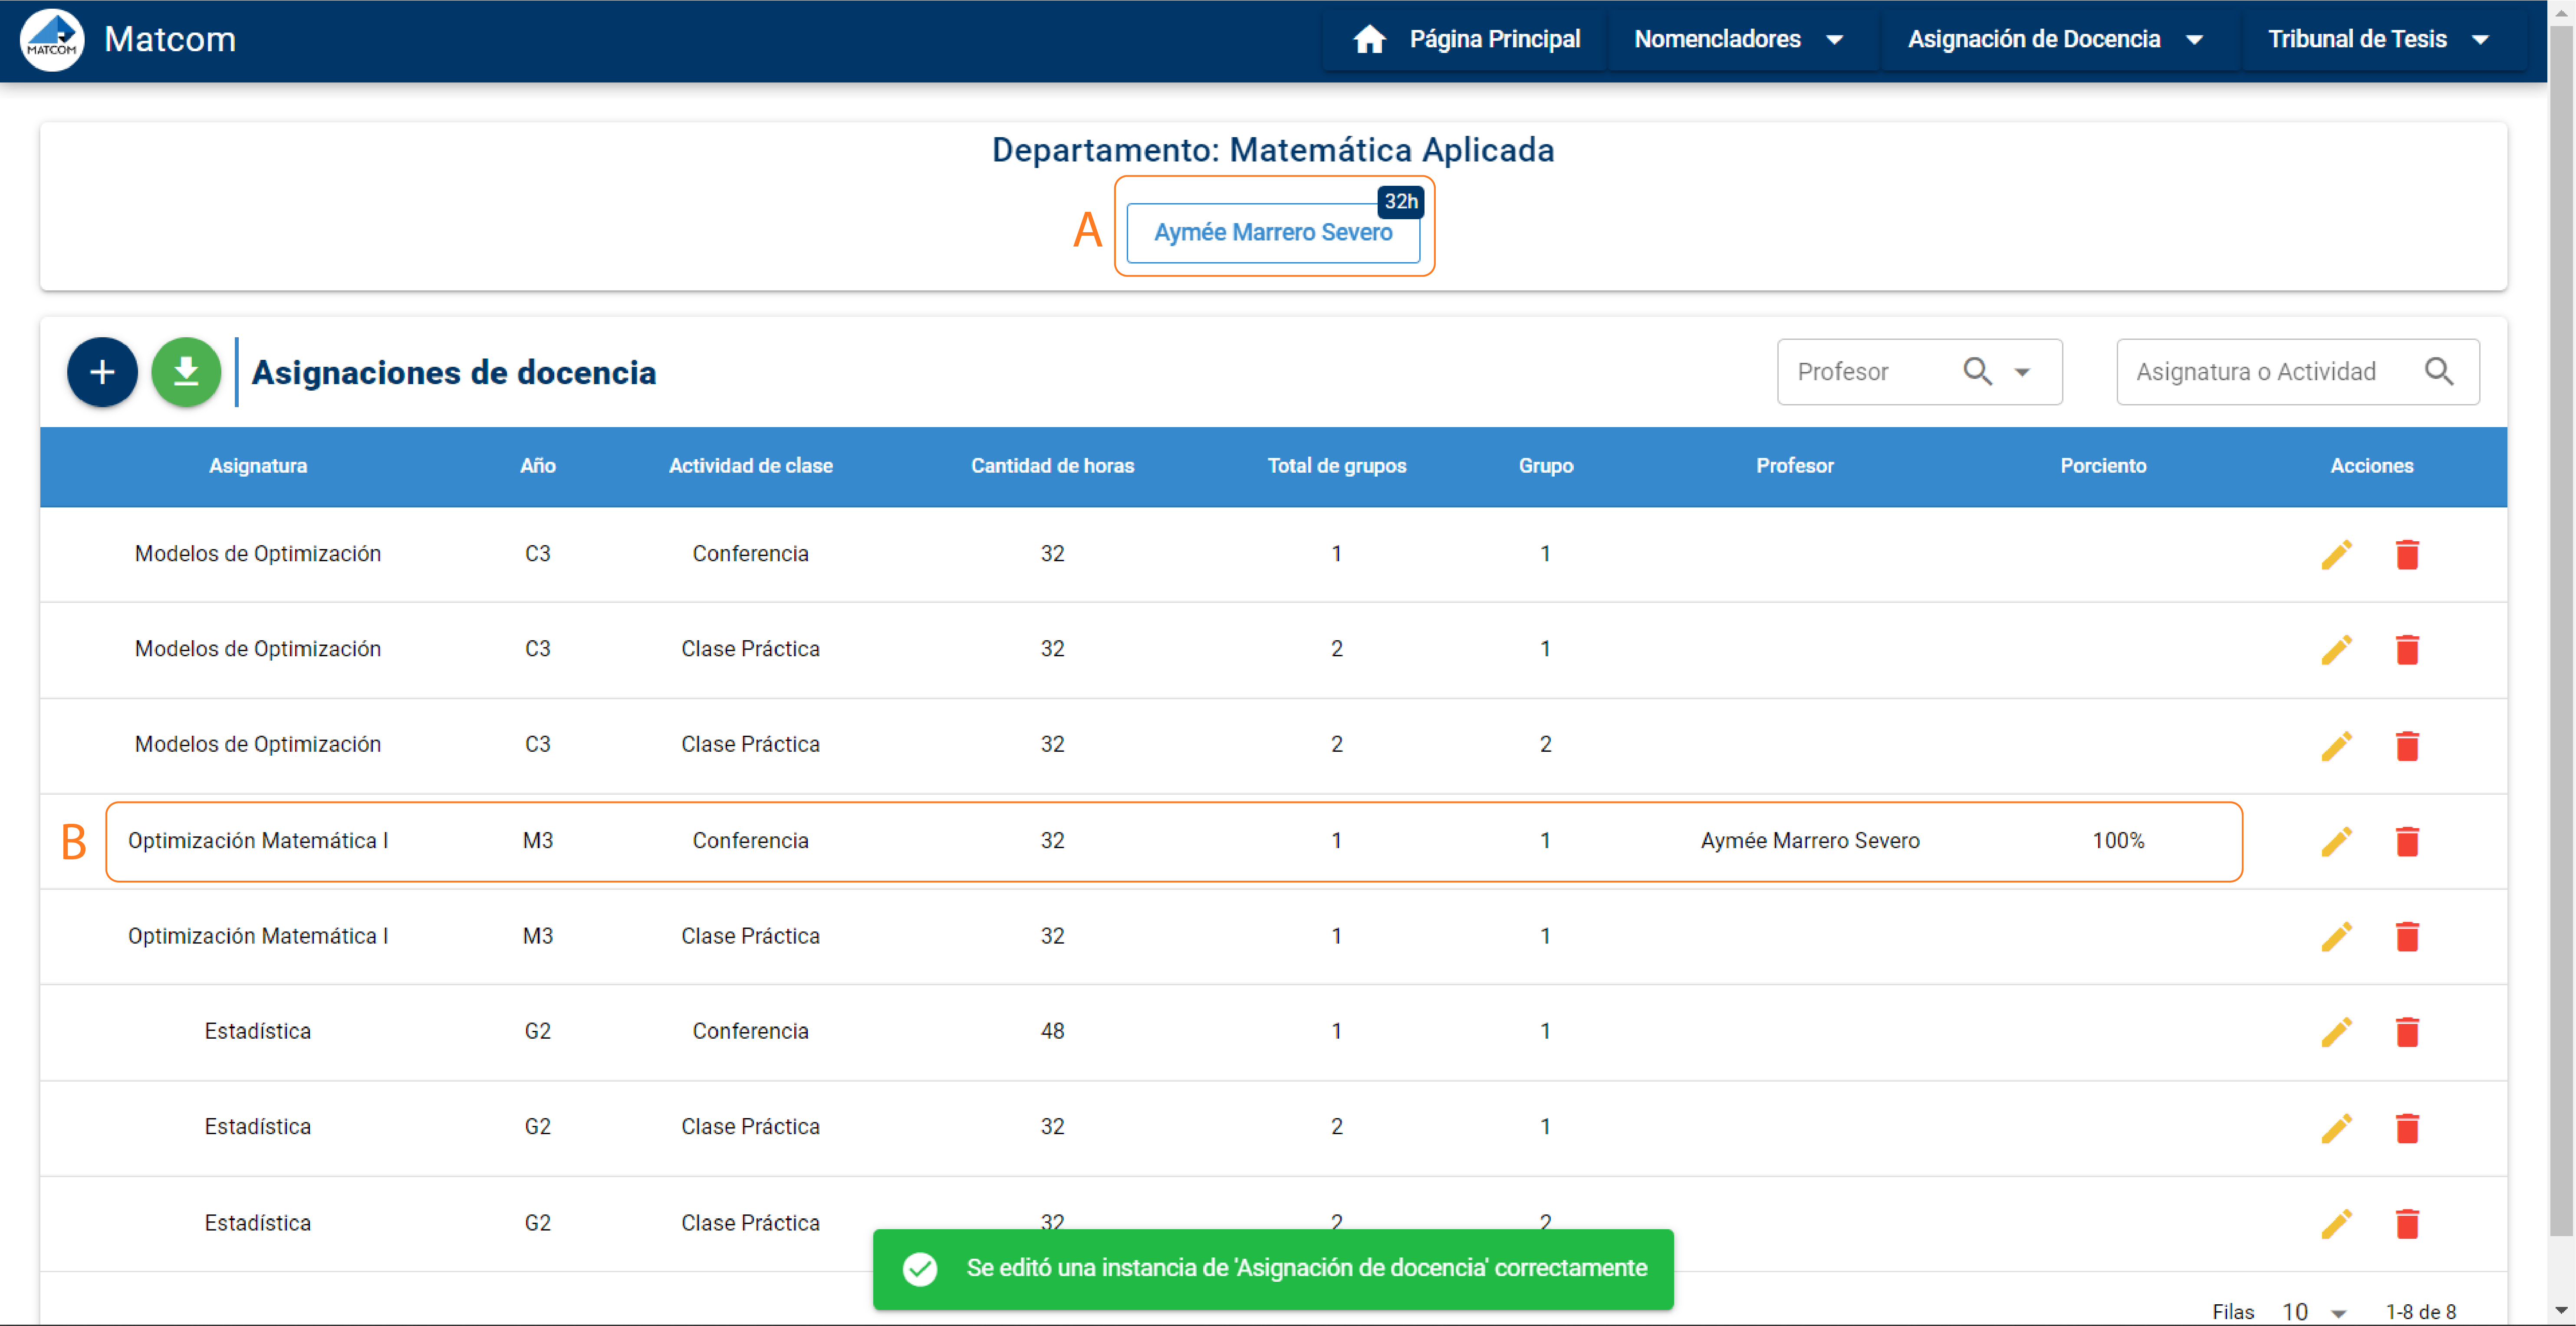
\includegraphics[scale=0.3]{Graphics/Implementation/Docencia/AD-one-assign.png}
    \caption{Vista resultante de realizar una asignación de docencia correctamente}
    \label{img-ta-one-assign}
\end{figure}

% Cada vez que se realicen cambios en la tabla, ya sean por agregar, editar o eliminar 
% asignaciones de docencia, la carga docente de los profesores se actualiza como se indica 
% en el recuadro A. El recuadro B refleja como quedó la fila tras la asignación de la profesora 
% Vivian Sistaschs para que imparta las 48 horas de conferencia de la asignatura Inferencia Matemática
% a los estudiantes que cursan el tercer año de la carrera Matemática.


Cada vez que se realicen cambios en la tabla, ya sean por agregar, editar o eliminar 
asignaciones de docencia, la carga docente de los profesores se actualiza como se indica 
en el recuadro A de la figura \ref{img-ta-one-assign}. El recuadro B refleja como quedó la fila tras la asignación de la profesora 
Aymée Marrero para que imparta las 32 horas de conferencia de la asignatura Optimización Matemática I
a los estudiantes que cursan el tercer año de la carrera Matemática.


En la figura \ref{img-ta-with-assign} se muestra el resultado de cubrir la docencia de las asignaturas de Optimización
Matemática I, Estadística y las clases prácticas de Modelos de Optimización, de acuerdo a la tabla \ref{tabla-asignación-cap4}.


\begin{figure}[H]
    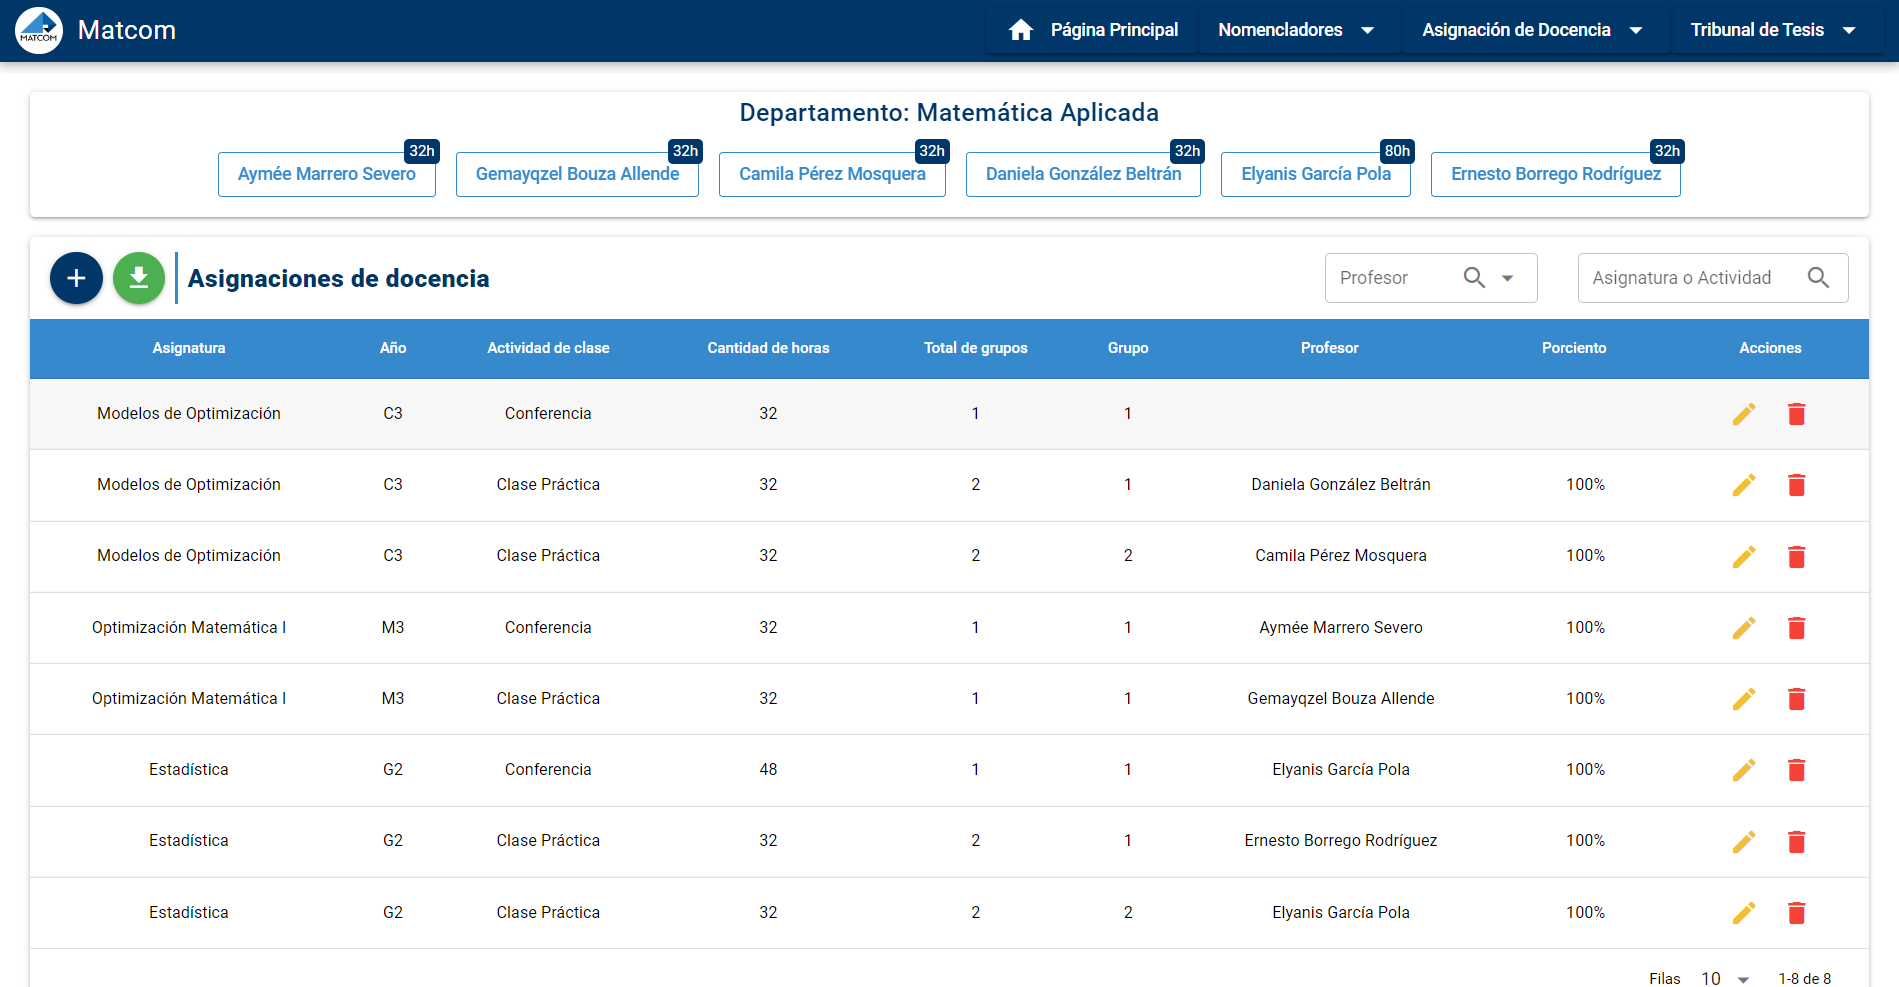
\includegraphics[scale=0.3]{Graphics/Implementation/Docencia/AD-with-assigns.png}
    \caption{Vista con varias asignaciones de docencia}
    \label{img-ta-with-assign}
\end{figure}


Las conferencias de la asignatura Modelos de Optimización I, se imparten por los profesores 
Aymée Marrero y Fernando Rodríguez, con 16 horas cada uno.
Para modelar esta distribución en el sistema, es necesario agregar una 
nueva asignación de docencia y especificar que cada profesor va a impartir el 50 porciento 
de las horas totales de conferencia. Para agregar una nueva asignación se debe pulsar sobre el 
botón de agregar y llenar los campos necesarios. En la figura
\ref{img-ta-result}, se muestra como queda
la asignación final de la docencia. 

\begin{figure}[H]
    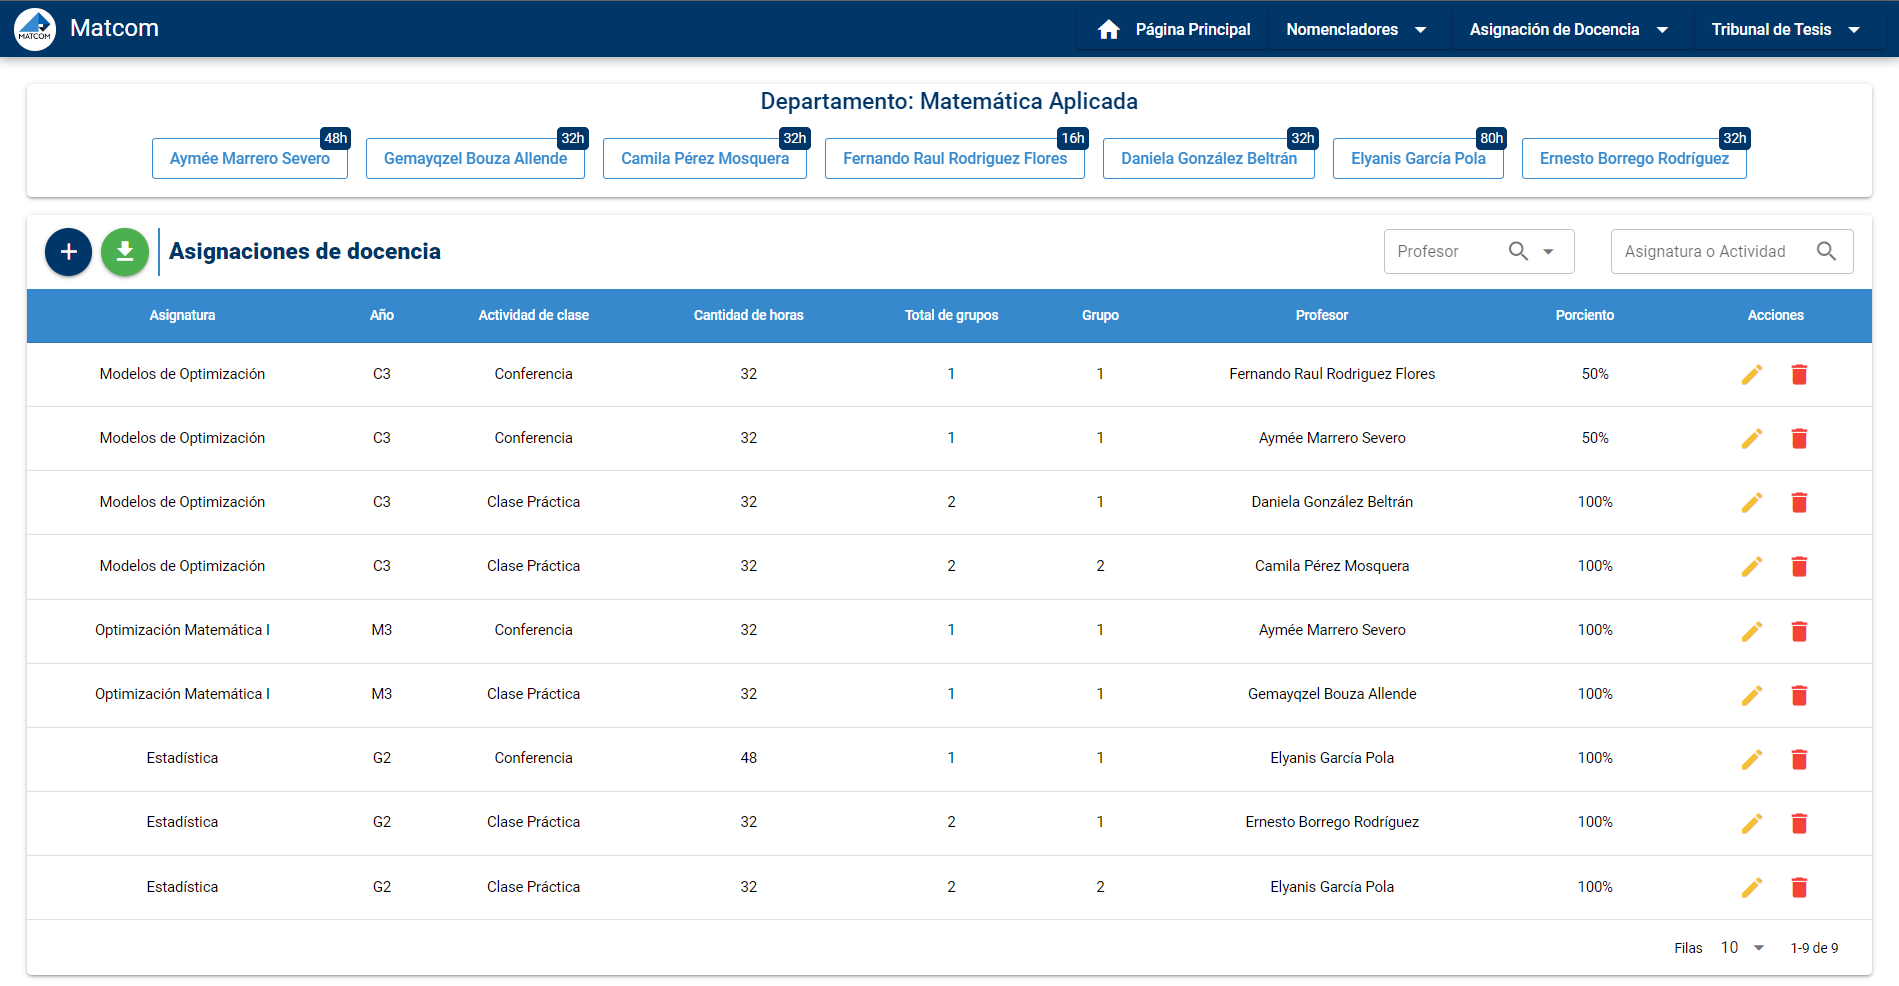
\includegraphics[scale=0.3]{Graphics/Implementation/Docencia/AD-result.png}
    \caption{Vista resultado de la asignaciones de docencia}
    \label{img-ta-result}
\end{figure}


Para poder llevar a cabo el proceso de asignación de docencia a través del sistema 
que se propone, es necesario que en la base de datos se ingresen las informaciones 
que intervienen en este proceso. Por ejemplo, para realizar una asignación de docencia se necesitan 
los profesores del departamento
y las planificaciones de las cargas de las asignaturas. Para poder crear las cargas  
se necesitan las asignaturas, los años escolares, las actividades de clase y los períodos de tiempo.
Por tanto el primer paso para realizar la asignación de docencia es ingresar todos los datos que 
se describen en la sección \ref{database:asignación-docencia}.







% El proceso de asignación de docencia en un departamento se realiza en la 
% interfaz que se muestra en la figura \ref{img-ta-done}. El usuario de la 
% aplicación puede ver la carga docente de los profesores durante el proceso 
% de asignación, realizar filtrados por profesor para ver las asignaturas 
% que tiene asignada y descargar un documento CSV que contiene la información 
% de la docencia una vez haya terminado la asignación.


% \begin{figure}[H]
%     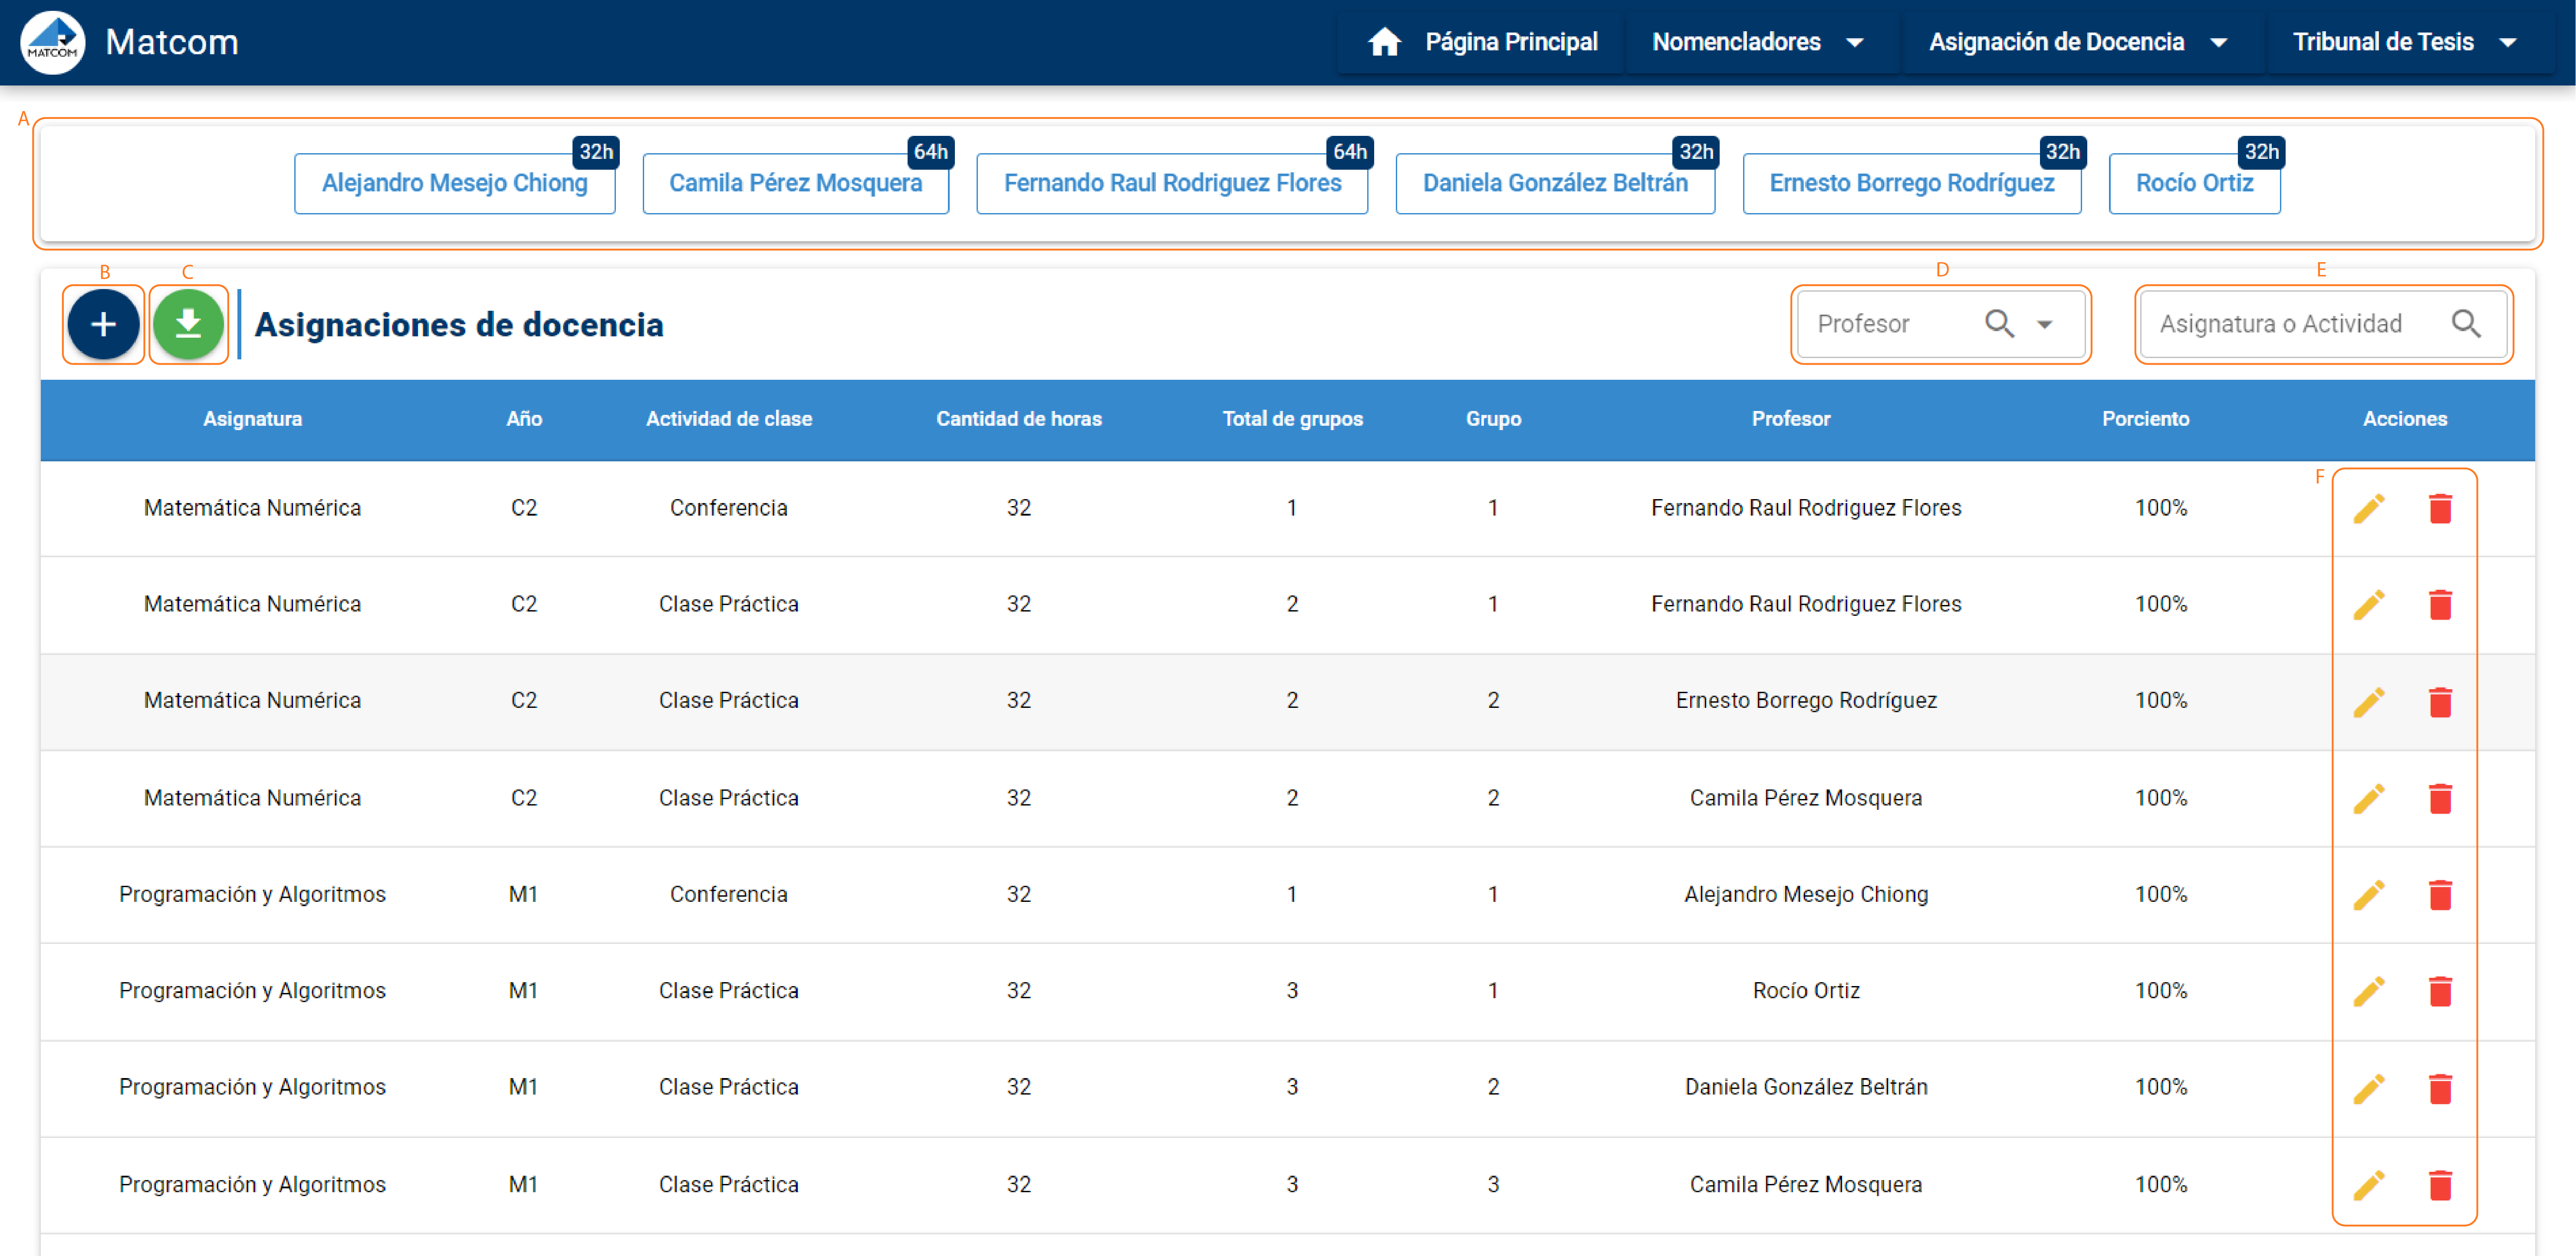
\includegraphics[scale=0.3]{Graphics/Implementation/Docencia/AD-asignada.png}
%     \caption{Vista de la asignación de docencia}
%     \label{img-ta-done}
% \end{figure}

% En la figura \ref{img-ta-done},
% se indican con recuadros cuatro regiones cuyo significado se explica a continuación.

% \begin{itemize}
%     \item A: muestra la carga docente de los profesores dada la asignación actual.
%     \item B: botón para agregar una nueva planificación de docencia.
%     \item C: botón para descargar la asignación de docencia actual.
%     \item D: realizar filtrado por los profesores para ver las asignturas que tiene asignadas.
%     \item E: realizar búsquedas por las asignaturas o actividades de clase.
%     \item F: botones para editar o borrar una fila de la tabla.  
% \end{itemize}



% En la figura \ref{img-ta-ordering} se muestra como quedaría ordenada la tabla a partir de los profesores,
% con el objetivo de mostrar primero aquellas 
% asignaturas que no se han asignado aún.


% \begin{figure}[H]
%     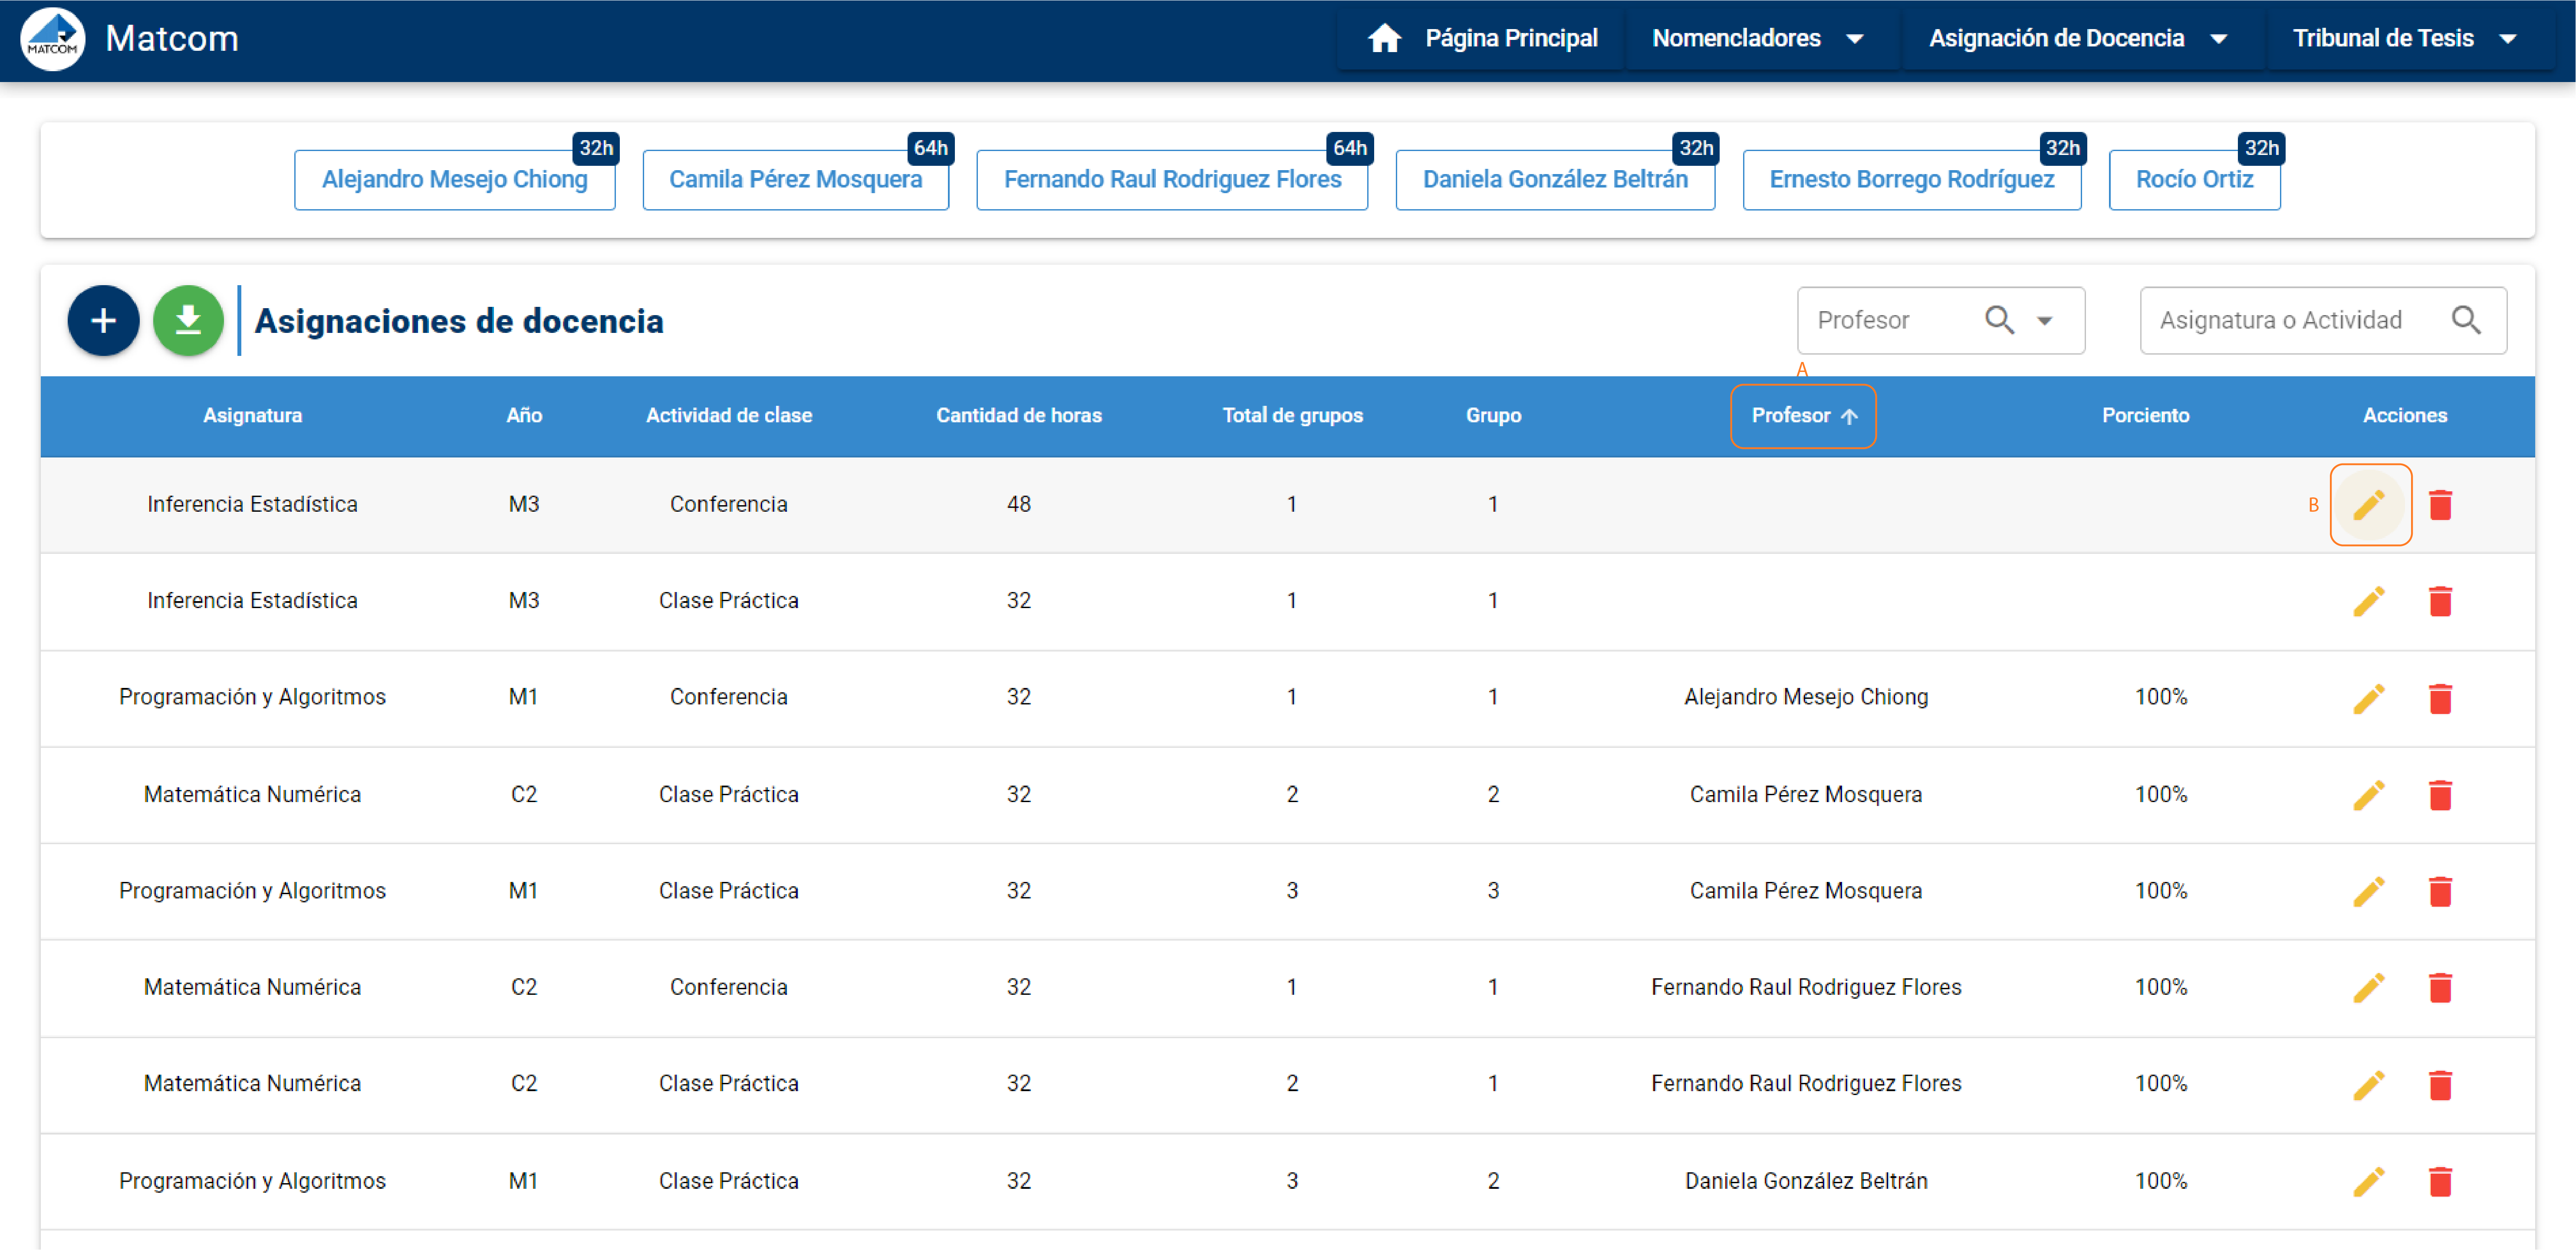
\includegraphics[scale=0.3]{Graphics/Implementation/Docencia/AD-sin-asignar.png}
%     \caption{Vista de la asignación de docencia, ordenada por profesores para que aparezcan primero las asignaturas que aún no han sido asignadas}
%     \label{img-ta-ordering}
% \end{figure}


% Para ordenar la tabla a partir de los profesores se debe pulsar sobre el elemento que se indica en 
% con el recuadro A. Para realizar una asignación se debe pulsar el botón de editar que se indica con
% con el recuadro B. La figura \ref{img-ta-edit-form1} muestra la vista después de pulsar el botón de 
% editar.  



% \begin{figure}[H]
%     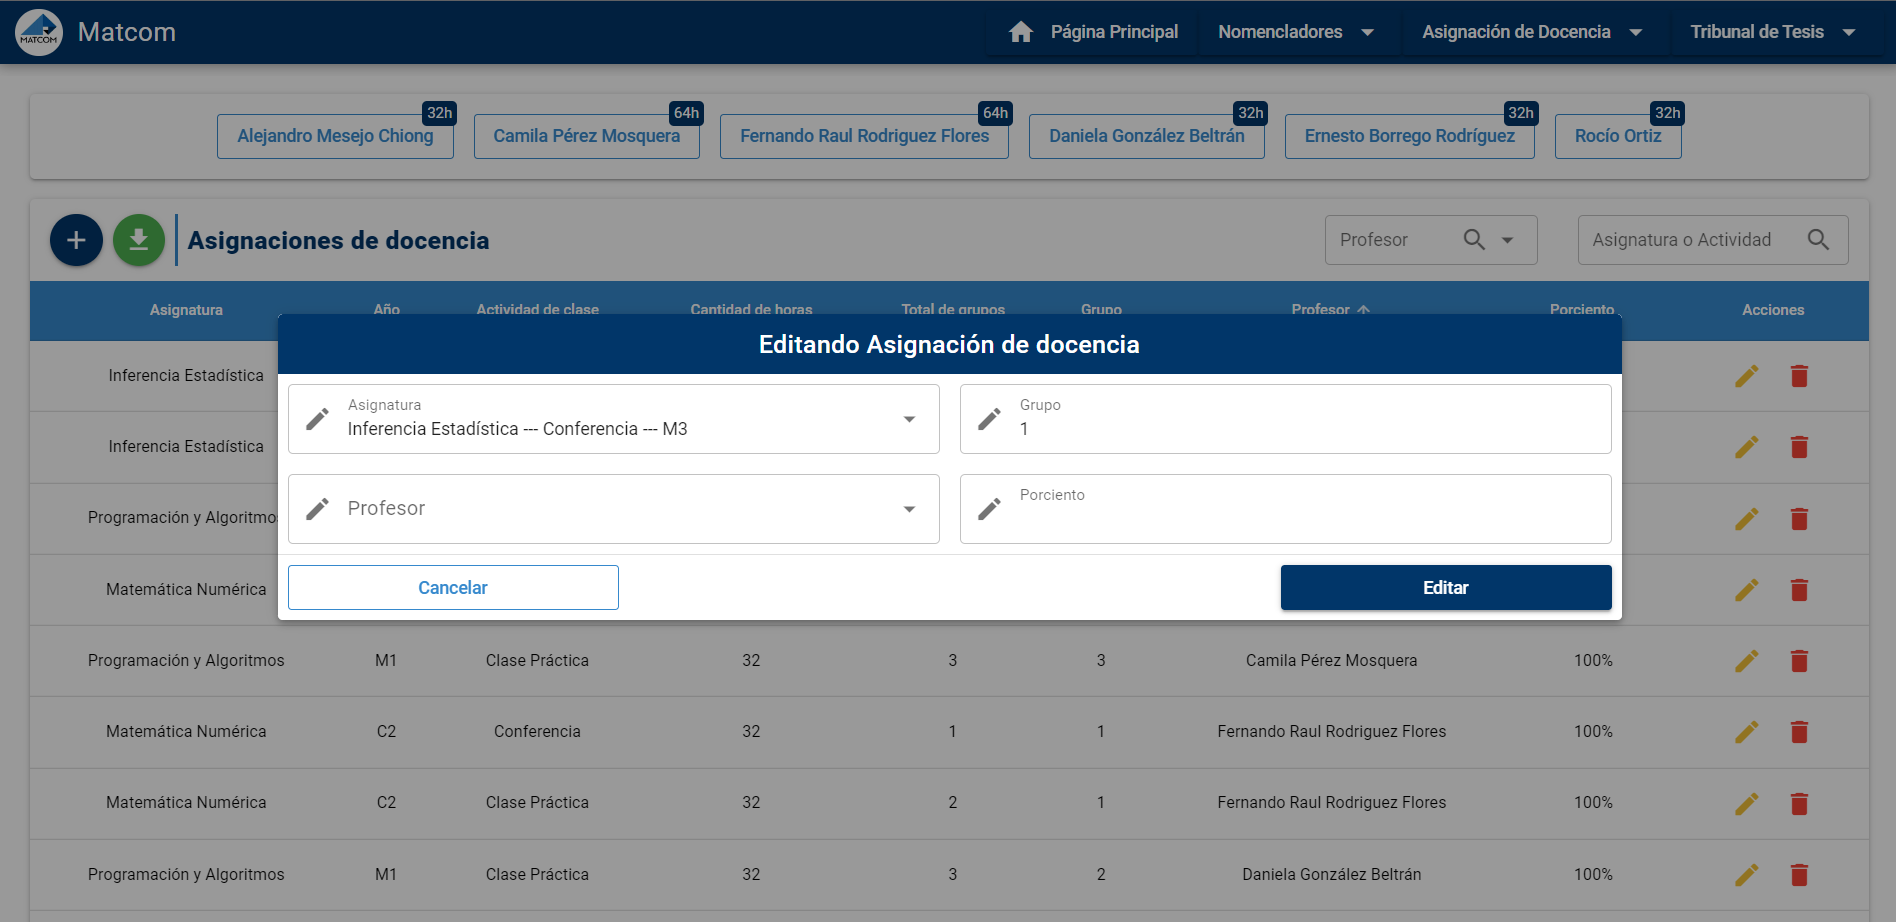
\includegraphics[scale=0.3]{Graphics/Implementation/Docencia/AD-edit-form.png}
%     \caption{Vista del formulario para editar una asignación de docencia}
%     \label{img-ta-edit-form1}
% \end{figure}


% Cuando se edita una asignación de docencia es necesario definir la planificación de 
% la asignatura (Inferencia Estadística---Conferencia---M3), grupo, profesor que se 
% desea asignar y el porciento total de horas que impartirá el profesor. En la figura
% \ref{img-ta-edit-form2} se muestra como asignar a la profesora Vivian Sistaschs con un 100
% porciento de las horas que se deben impartir en la planificación de la asignatura Inferencia Estadística. 

% \begin{figure}[H]
%     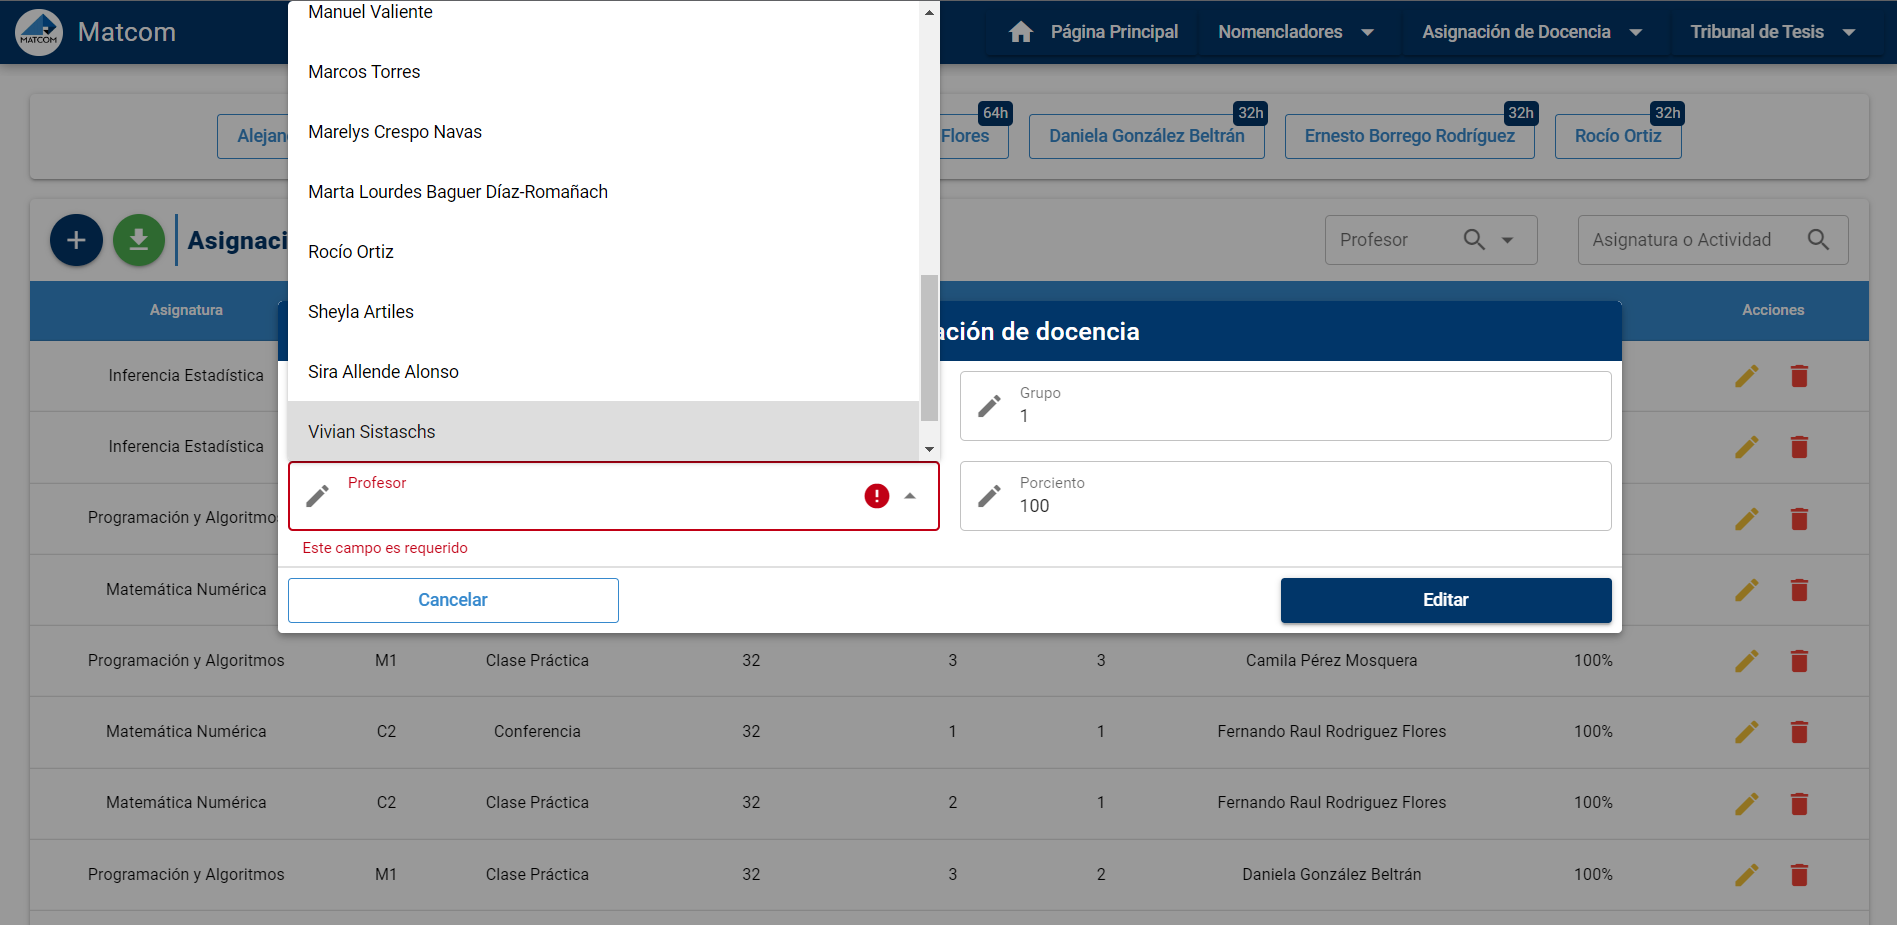
\includegraphics[scale=0.3]{Graphics/Implementation/Docencia/AD-edit-form2.png}
%     \caption{Vista del formulario para editar una asignación de docencia, mostrando los profesores posibles para la asignación}
%     \label{img-ta-edit-form2}
% \end{figure}



% La figura \ref{img-ta-result} muestra el resultado de completar los pasos
% que se muestran en la figuras \ref{img-ta-ordering}, \ref{img-ta-edit-form1} y \ref{img-ta-edit-form2}.

% % \begin{figure}[H]
% %     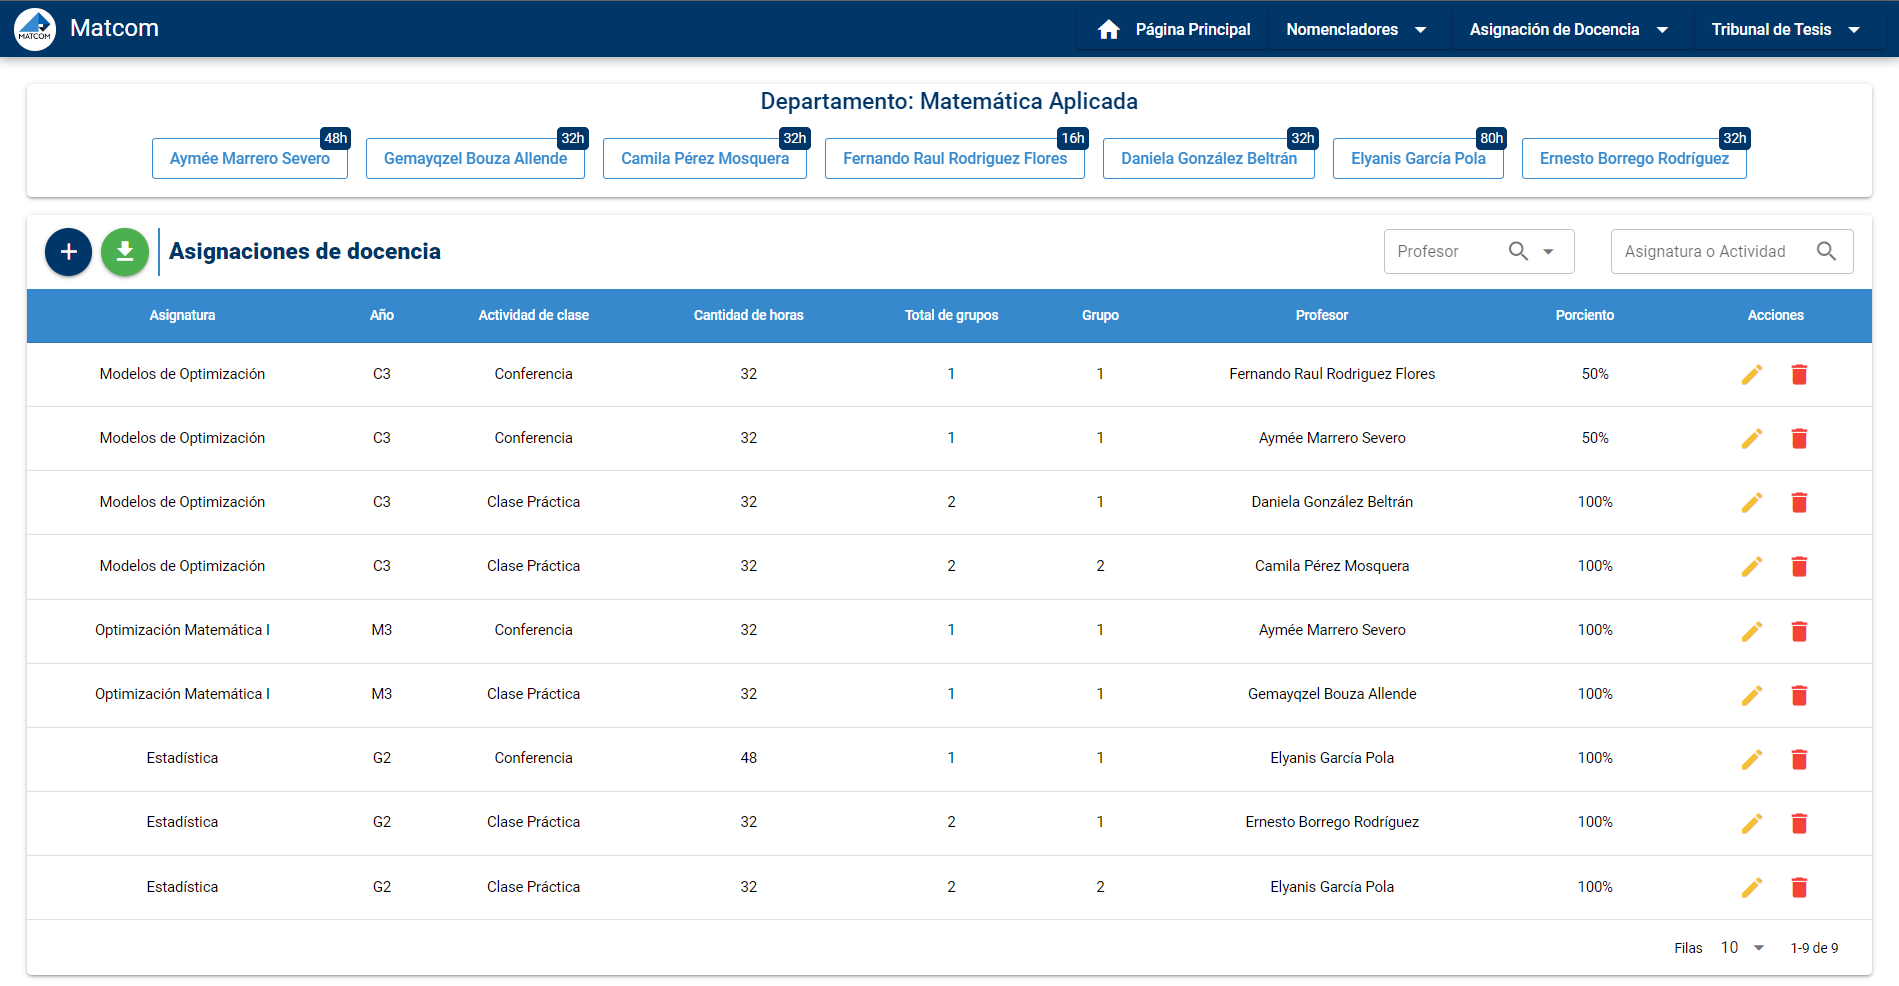
\includegraphics[scale=0.3]{Graphics/Implementation/Docencia/AD-result.png}
% %     \caption{Vista de la asignación tras realizar una asignación correctamente}
% %     \label{img-ta-result}
% % \end{figure}

% Cada vez que se realicen cambios en la tabla, ya sean por agregar, editar o eliminar 
% asignaciones de docencia, la carga docente de los profesores se actualiza como se indica 
% en el recuadro A. El recuadro B refleja como quedó la fila tras la asignación de la profesora 
% Vivian Sistaschs para que imparta las 48 horas de conferencia de la asignatura Inferencia Matemática
% a los estudiantes que cursan el tercer año de la carrera Matemática.



En la siguiente sección se describen los pasos para realizar la confección de los 
tribunales y la planificación de las defensas de tesis.

\section{Planificación de las tesis} \label{cap4:tesis}
La planificación de las tesis consta de dos subprocesos principales: la confección de los tribunales 
y la programación de las defensas. 
En esta sección se describen los pasos a seguir para completar 
la planificación de las tesis a través del sistema.
Para ilustrar este proceso se utilizará el mismo ejemplo que se 
describe en la sección \ref{tesis:cap2}. 
En la tabla \ref{tabla-tesis-cap4} se muestran los datos de dos 
tesis, en la tabla \ref{tabla-tribunal-tesis-cap2} el tribunal seleccionado y en 
la tabla \ref{tabla-defensa-tesis-cap4} el horario escogido para la defensa de las mismas.

\begin{table}[H]
    \centering
    \begin{tabular}{ | c | c | c | c |}
      \hline
      \thead{ID} & \thead{Tesis} & \thead{Estudiante} & \thead{Tutores} \\
      \hline 
             1 & \makecell{Simulación y optimización \\ de movimientos de malabares} & Gustavo Despaigne & Fernando Rodríguez  \\
      \hline
             2 & \makecell{Propagación de epidemias \\ mediante modelos basados \\ en metapoblaciones} & Abel Antonio Cruz & \makecell{Angela M. León \\ José A. Mesejo} \\
      \hline
    \end{tabular}
    \caption{Datos de las tesis}
    \label{tabla-tesis-cap4}
\end{table}


\begin{table}[H]
    \centering
    \begin{tabular}{ | c | c | c | c |}
      \hline
      \thead{ID Tesis} & \thead{Tutores} & \thead{Oponente} & \thead{Presidente} \\
      \hline 
             1 & Fernando Rodríguez & Gemayqzel Bouza & Aymée Marrero  \\
      \hline
             2 & \makecell{Angela M. León \\ José A. Mesejo } & Damian Valdés & Gemayqzel Bouza  \\
      \hline
    \end{tabular}
    \caption{Posibles tribunales para las tesis tesis}
    \label{tabla-tribunal-tesis-cap4}
\end{table}

\begin{table}[H]
    \centering
    \begin{tabular}{ | c | c | c | c |}
      \hline
      \thead{ID Tesis} & \thead{Fecha} & \thead{Hora} & \thead{Local} \\
      \hline 
             1 & 10/12/2022 & 2:00 PM & Aula Posgrado  \\
      \hline
             2 & 10/12/2022 & 3:30 PM & Salón del Decanato \\
      \hline
    \end{tabular}
    \caption{Posible horarios para los actos de defensa}
    \label{tabla-defensa-tesis-cap4}
\end{table}


El primer paso es ingresar las tesis en el sistema,
en la figura \ref{img-tc-thesis} se muestra la interfaz de usuario
que permite realizar esta tarea.


\begin{figure}[H]
    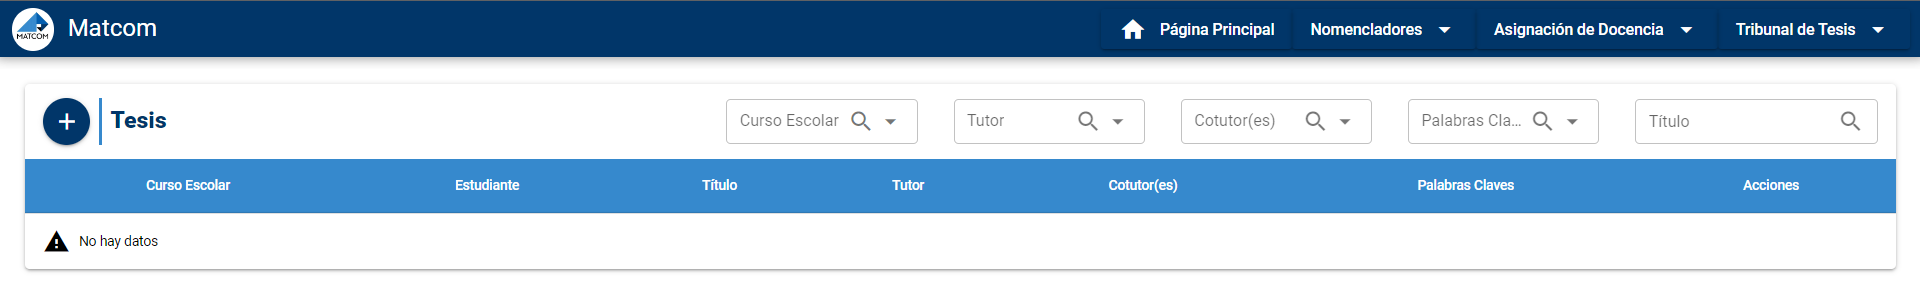
\includegraphics[scale=0.3]{Graphics/Implementation/Tesis/thesis-empty.png}
    \caption{Vista de la tesis.}
    \label{img-tc-thesis}
\end{figure}


Para agregar una nueva tesis en el sistema, se debe pulsar sobre el botón 
de agregar que se indica en el recuadro A de la figura \ref{img-tc-thesis}.
Luego se deben llenar los campos necesarios relacionados con las tesis. En la figura
\ref{img-tc-thesis-form} se muestra el resultado de pulsar sobre el botón de agregar y llenar los campos 
correspondientes a la primera tesis que se muestra en la tabla \ref{tabla-tesis-cap4}.

\begin{figure}[H]
    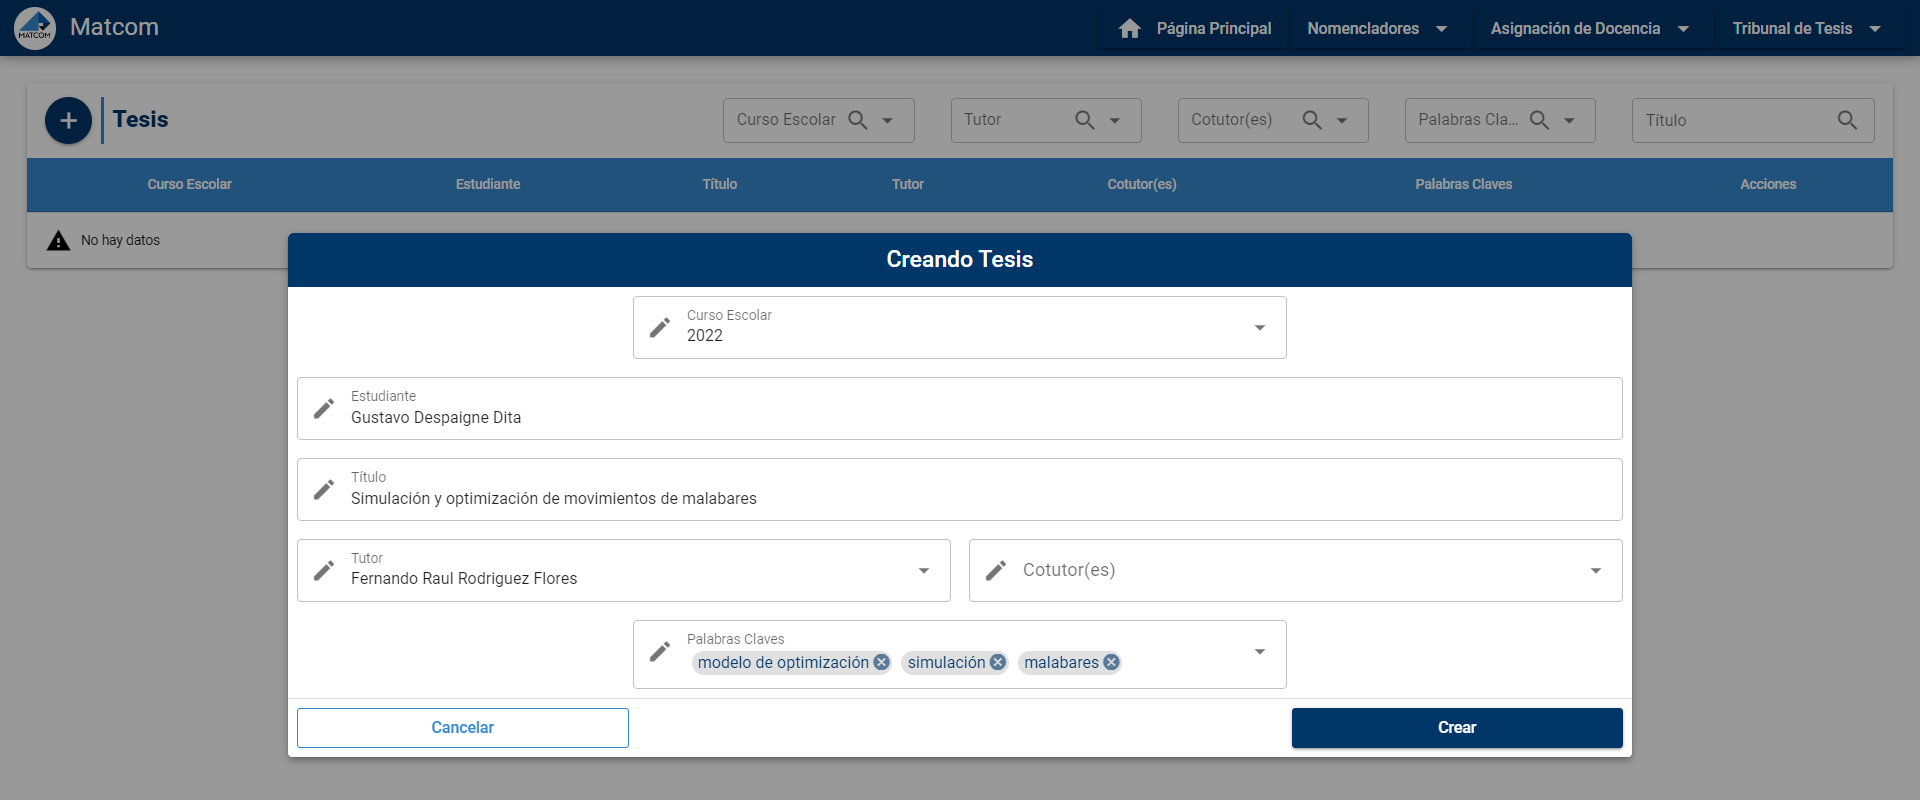
\includegraphics[scale=0.3]{Graphics/Implementation/Tesis/thesis-form.png}
    \caption{Vista del formulario para agregar una tesis.}
    \label{img-tc-thesis-form}
\end{figure}


Repitiendo el procedimiento anterior se puede agregar la segunda tesis que se 
muestra en la tabla \ref{tabla-tesis-cap4}. En la figura \ref{img-tc-thesis-result} tal
se muestra el resultado de agregar las dos tesis en el sistema.

\begin{figure}[H]
    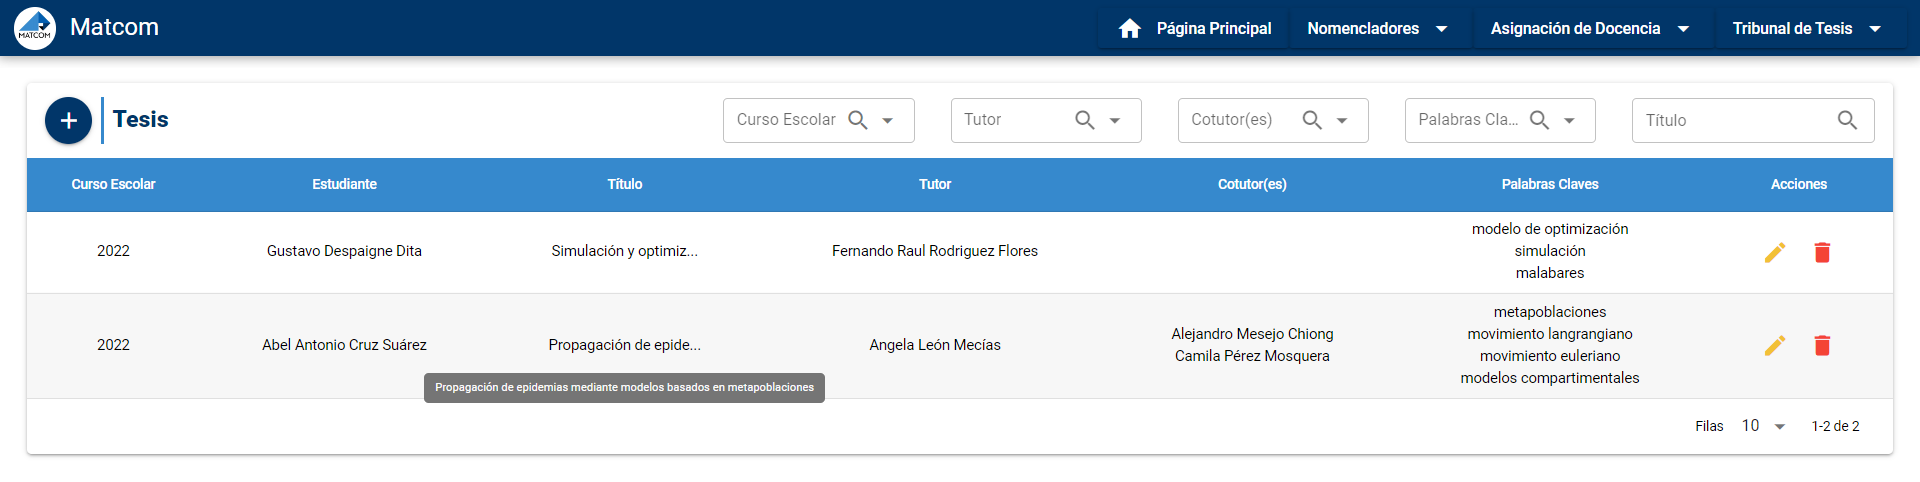
\includegraphics[scale=0.3]{Graphics/Implementation/Tesis/thesis-result.png}
    \caption{Vista de la interfaz de usuario tras agregar las dos tesis del ejemplo.}
    \label{img-tc-thesis-result}
\end{figure}

Cada vez que se agregue una tesis al sistema, se crea una  
instancia de un tribunal de tesis con los campos de oponente y presidente sin asignar.
En la figura \ref{img-tc-thesis-committee-empty}  se muestran los tribunales incompletos creados 
automáticamente a partir de las tesis que se ingresaron en el sistema.

\begin{figure}[H]
    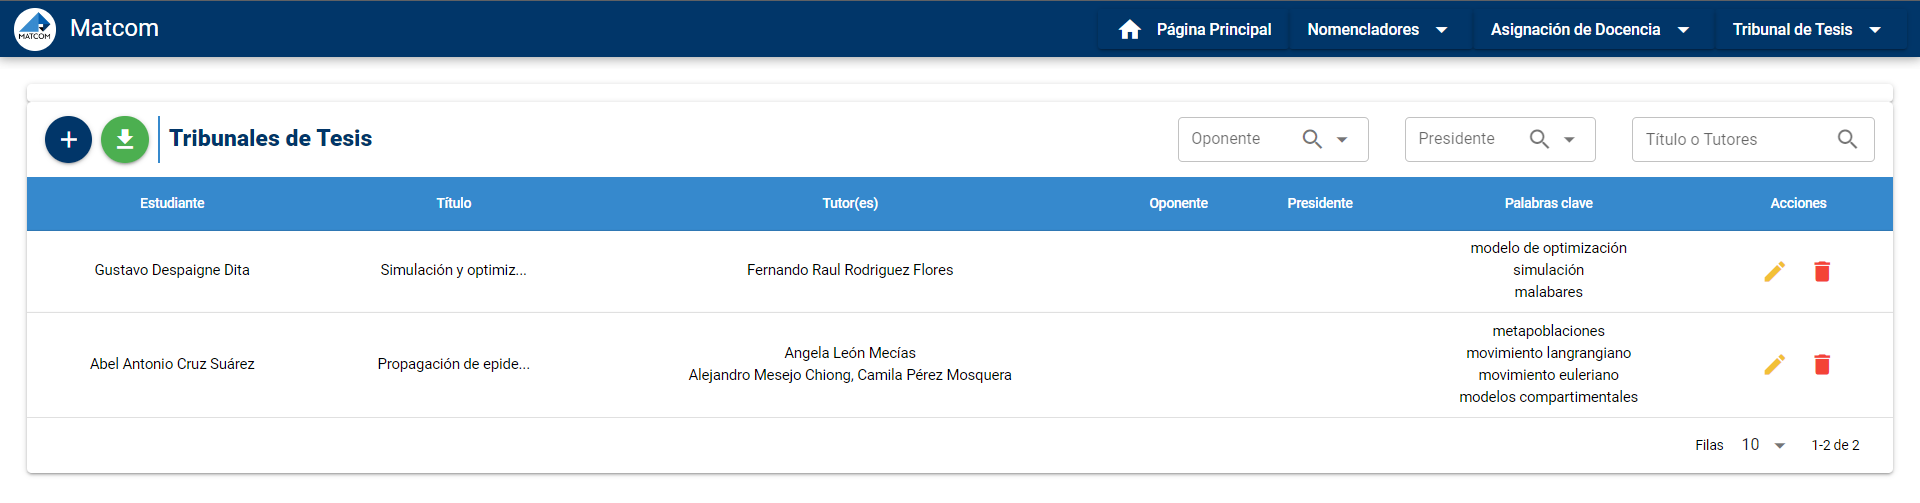
\includegraphics[scale=0.3]{Graphics/Implementation/Tesis/thesis-committee-empty.png}
    \caption{Vista de la interfaz de usuario para la confección de los tribunales.}
    \label{img-tc-thesis-committee-empty}
\end{figure}


El próximo paso es asignar los profesores que conformarán  los tribunales de tesis.
El encargado de realizar este proceso debe pulsar sobre el botón de editar 
de la fila correspondiente al tribunal que desea definir. En la figura \ref{img-tc-thesis-committee-form}
se muestra el resultado de pulsar sobre el botón de la primera fila y completar el tribunal
con los profesores que se muestran en la tabla \ref{tabla-tribunal-tesis-cap4}.


\begin{figure}[H]
    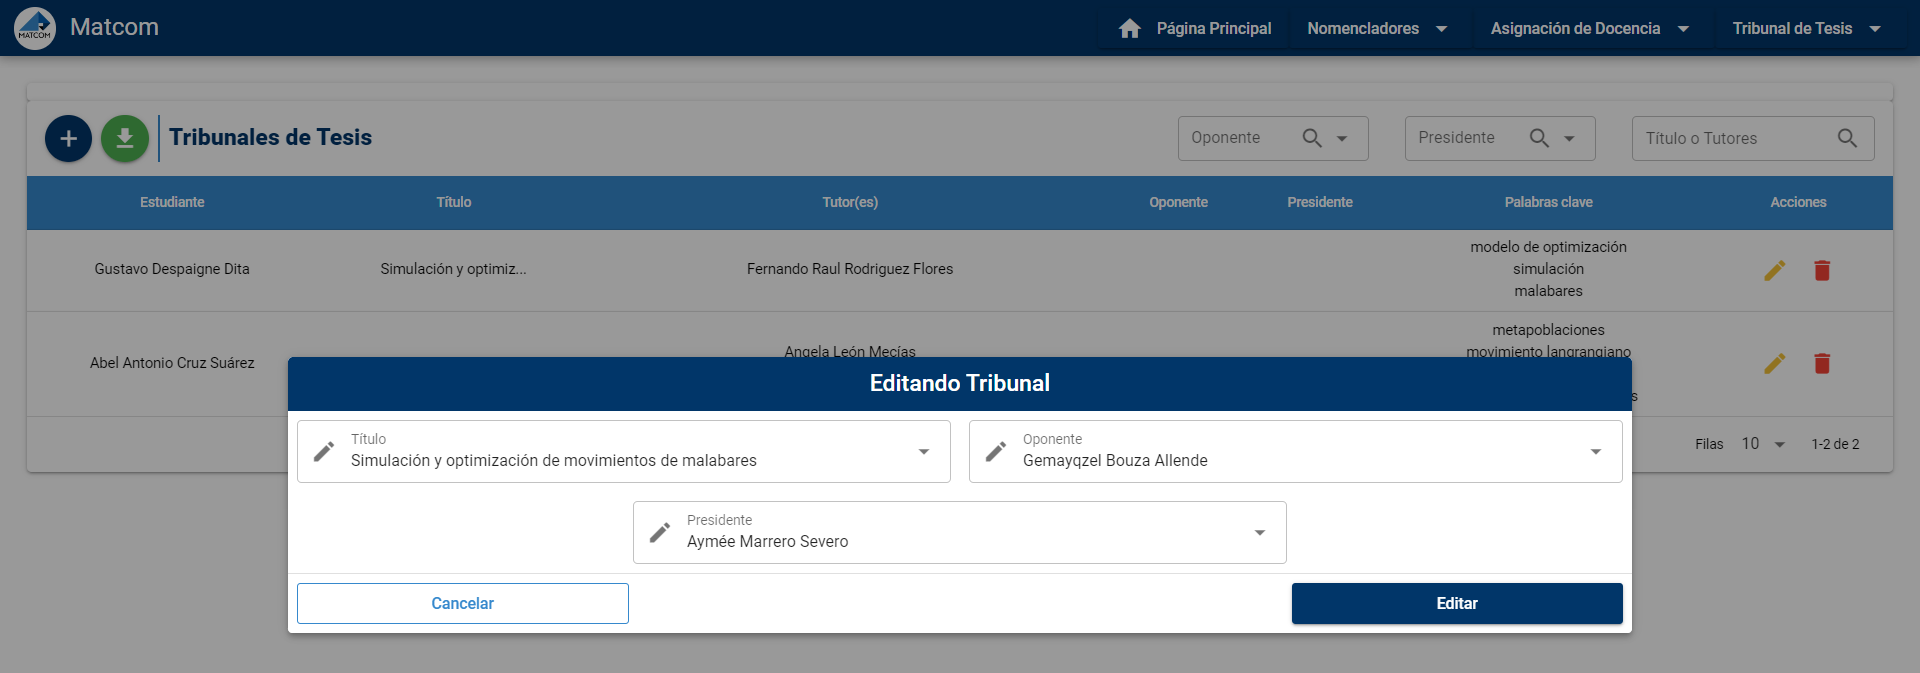
\includegraphics[scale=0.3]{Graphics/Implementation/Tesis/thesis-committee-form.png}
    \caption{Vista del formulario para la confección de los tribunales.}
    \label{img-tc-thesis-committee-form}
\end{figure}


Cada vez que un tribunal de tesis se modifique se actualiza la participación de los 
profesores en tribunales, para cada profesor se muestra la cantidad de tribunales en los que 
participa como oponente y como presidente. En la figura \ref{img-tc-thesis-committee-assign1}
se muestra el resultado de confeccionar el tribunal para la tesis del estudiante Gustavo Despaigne 
Dita.


\begin{figure}[H]
    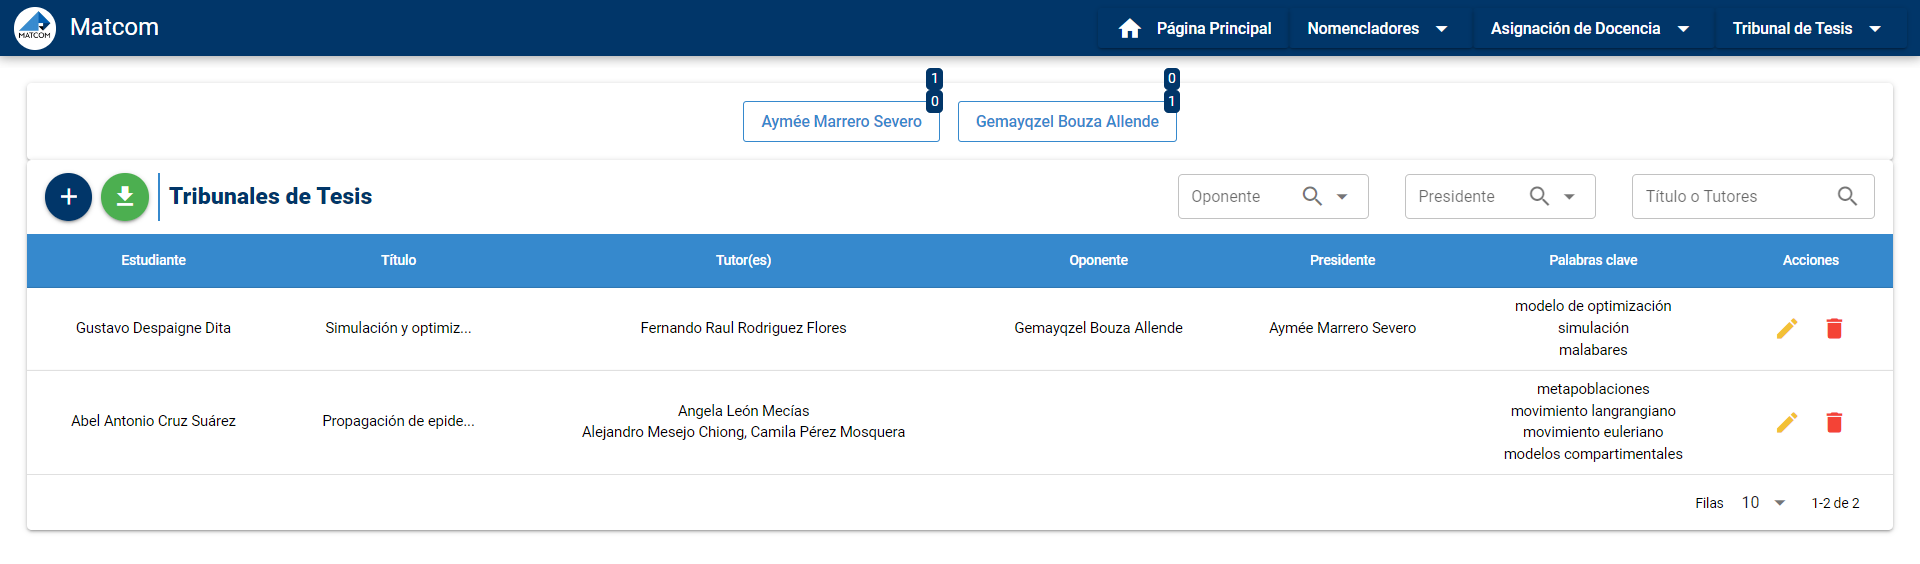
\includegraphics[scale=0.3]{Graphics/Implementation/Tesis/thesis-committee-assign1.png}
    \caption{Vista resultante de confeccionar el tribunal de la primera tesis de la tabla.}
    \label{img-tc-thesis-committee-assign1}
\end{figure}

En el recuadro A que se indica en la figura \ref{img-tc-thesis-committee-assign1},
se muestran las participaciones de los profesores en los tribunales que se hayan asignado.
En este ejemplo, la profesora Aymée Marrero participa en 0 tribunales como oponente y en 1 tribunal
como presidente y la profesora Gemayqzel Bouza participa en 1 tribunal como oponente y en 0 tribunales 
como presidente.
El recuadro B muestra una descripción que aparece al colocar el cursor sobre uno de los profesores, en 
este caso sobre el recuadro que representa la cantidad de tribunales en los que participa la profesora Gemayqzel.
La figura \ref{img-tc-thesis-committee-assign2} muestra el resultado de confeccionar el tribunal para la tesis del estudiante Abel
Antonio Cruz Suárez.

\begin{figure}[H]
    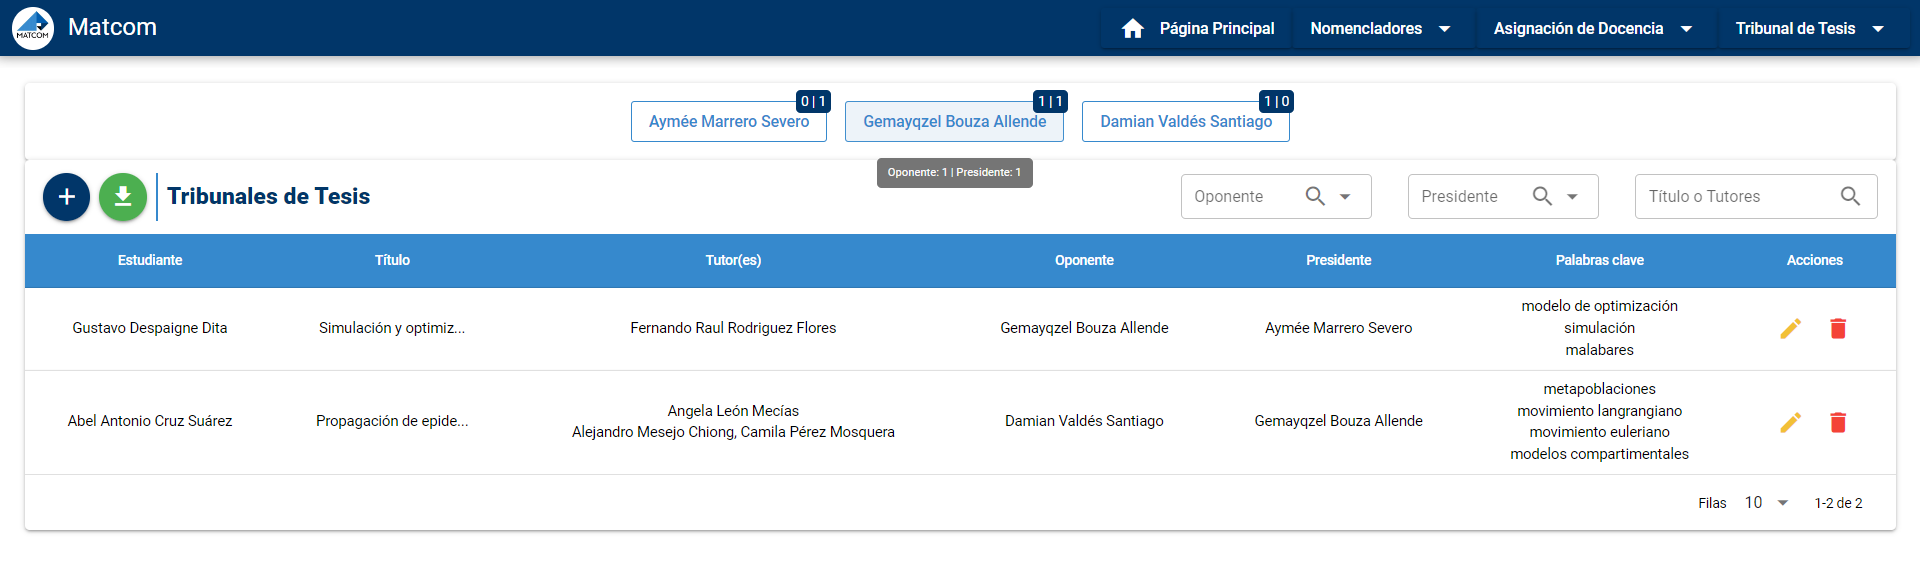
\includegraphics[scale=0.3]{Graphics/Implementation/Tesis/thesis-committee-assign2.png}
    \caption{Vista del formulario para la confección de los tribunales.}
    \label{img-tc-thesis-committee-assign2}
\end{figure}

En la figura \ref{img-tc-thesis-committee-assign2}
se puede apreciar que se actualizaron las participaciones de los profesores en los tribunales.
Se agregó la participación del profesor Damian Valdés y se actualizó la de la profesora Gemayqzel Bouza, 
aumentando en 1 la cantidad de participaciones en tribunales como presidente.


Cuando se hayan confeccionado los tribunales de tesis, el siguiente paso 
es realizar la programación de las defensas. 
Cuando una tesis se agrega al sistema, se crea una instancia 
de una defensa de tesis sin definir los campos fecha, hora y local.
En la figura \ref{img-tc-thesis-defense-empty} se muestra la interfaz de usuario donde se realiza 
el proceso de programación de las defensas.

\begin{figure}[H]
    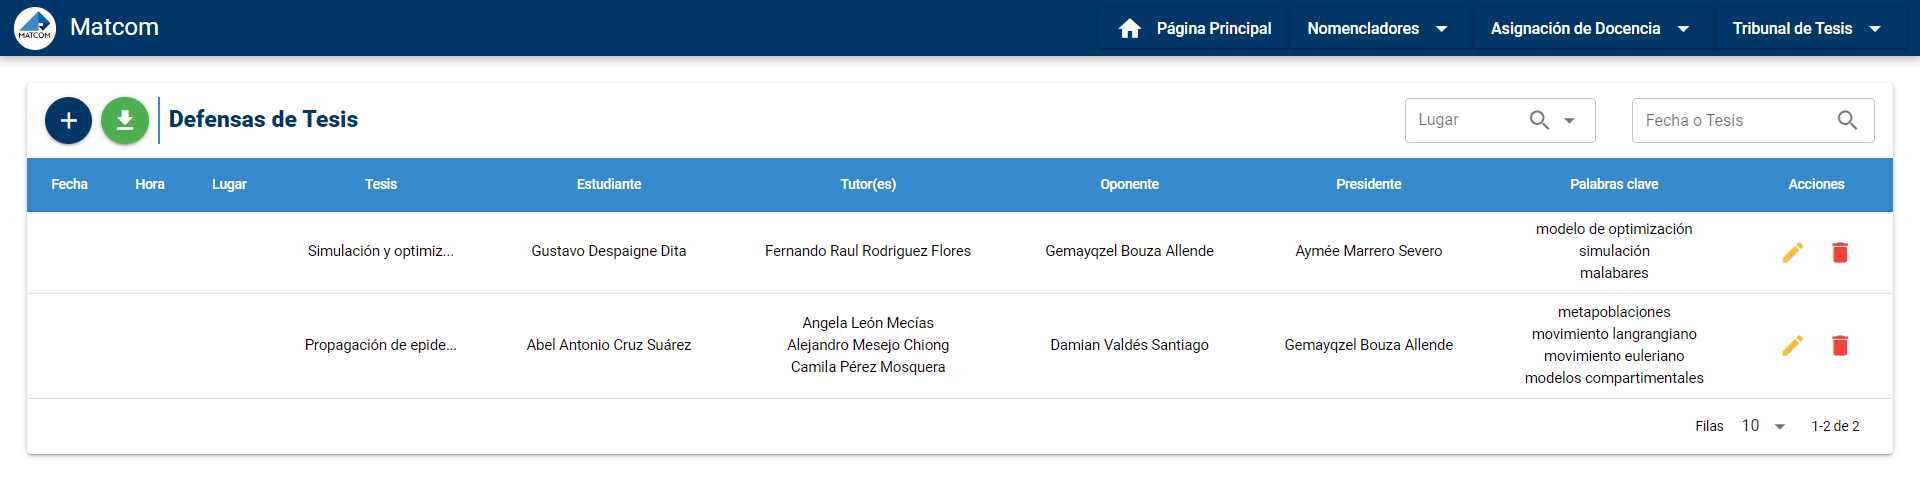
\includegraphics[scale=0.3]{Graphics/Implementation/Tesis/thesis-defense-empty.png}
    \caption{Interfaz de usario para programar las defensas de tesis}
    \label{img-tc-thesis-defense-empty}
\end{figure}

Similar al proceso de confección de los tribunales, para definir la fecha, hora y lugar 
donde se realizará la defensa de una tesis, se debe pulsar sobre el botón de editar correspondiente 
a la fila de la defensa que se desea planificar. En la figura \ref{img-tc-thesis-defense-form}
se muestra el resultado de pulsar sobre el botón de editar de la primera fila
y completar los datos de la planificación correspondiente a la tabla \ref{tabla-defensa-tesis-cap4}. 


\begin{figure}[H]
    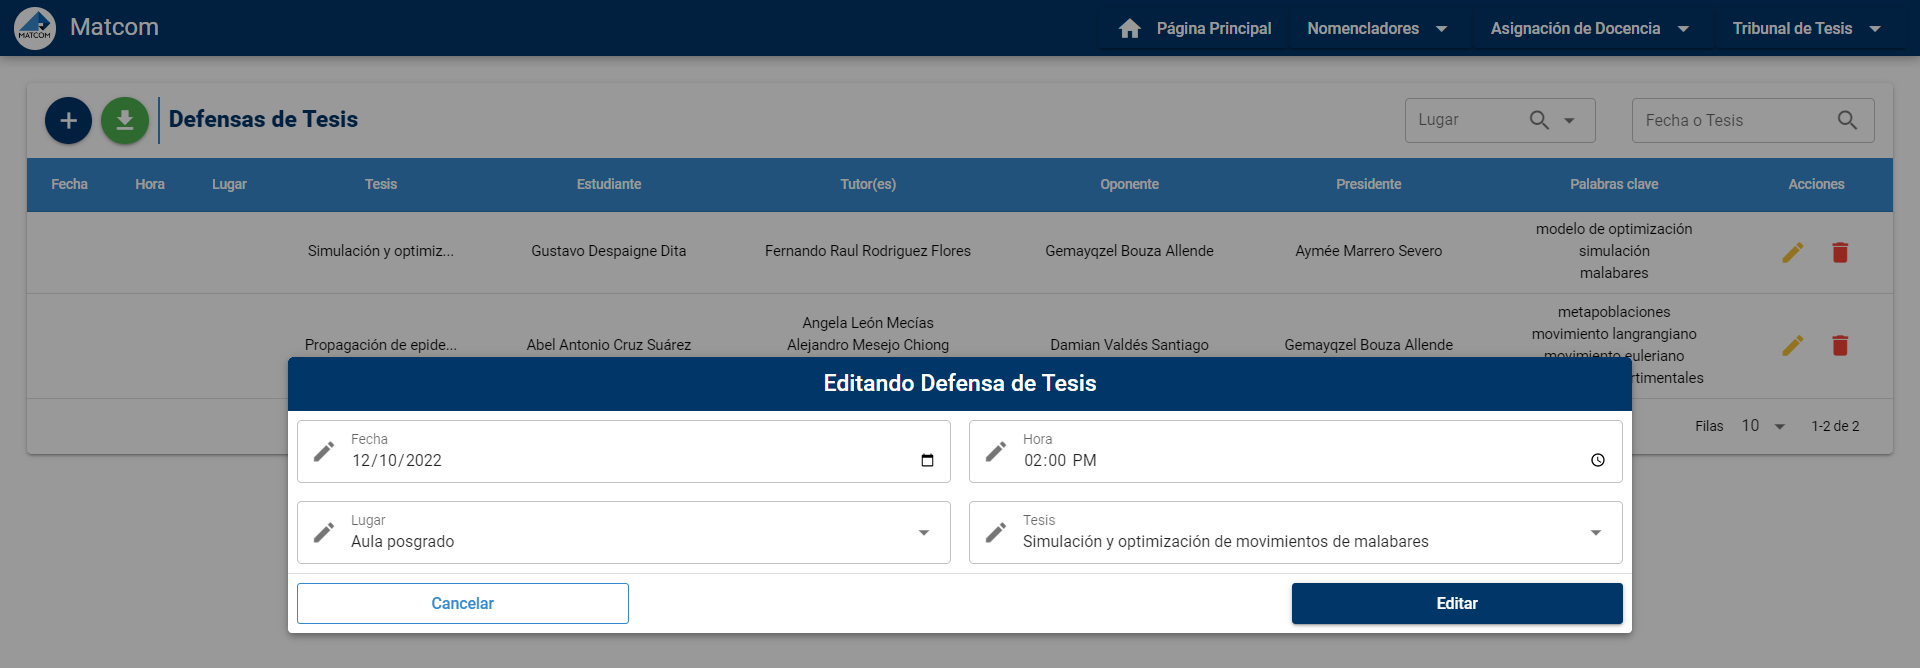
\includegraphics[scale=0.3]{Graphics/Implementation/Tesis/thesis-defense-form.png}
    \caption{Vista del formulario para la planificación de las tesis.}
    \label{img-tc-thesis-defense-form}
\end{figure}


Una vez que se hayan programado las defensas de las tesis, se puede 
exportar la información de estas a un archivo CSV pulsando sobre el recuadro A que se 
muestra en la figura \ref{img-tc-thesis-defense-result}.


\begin{figure}[H]
    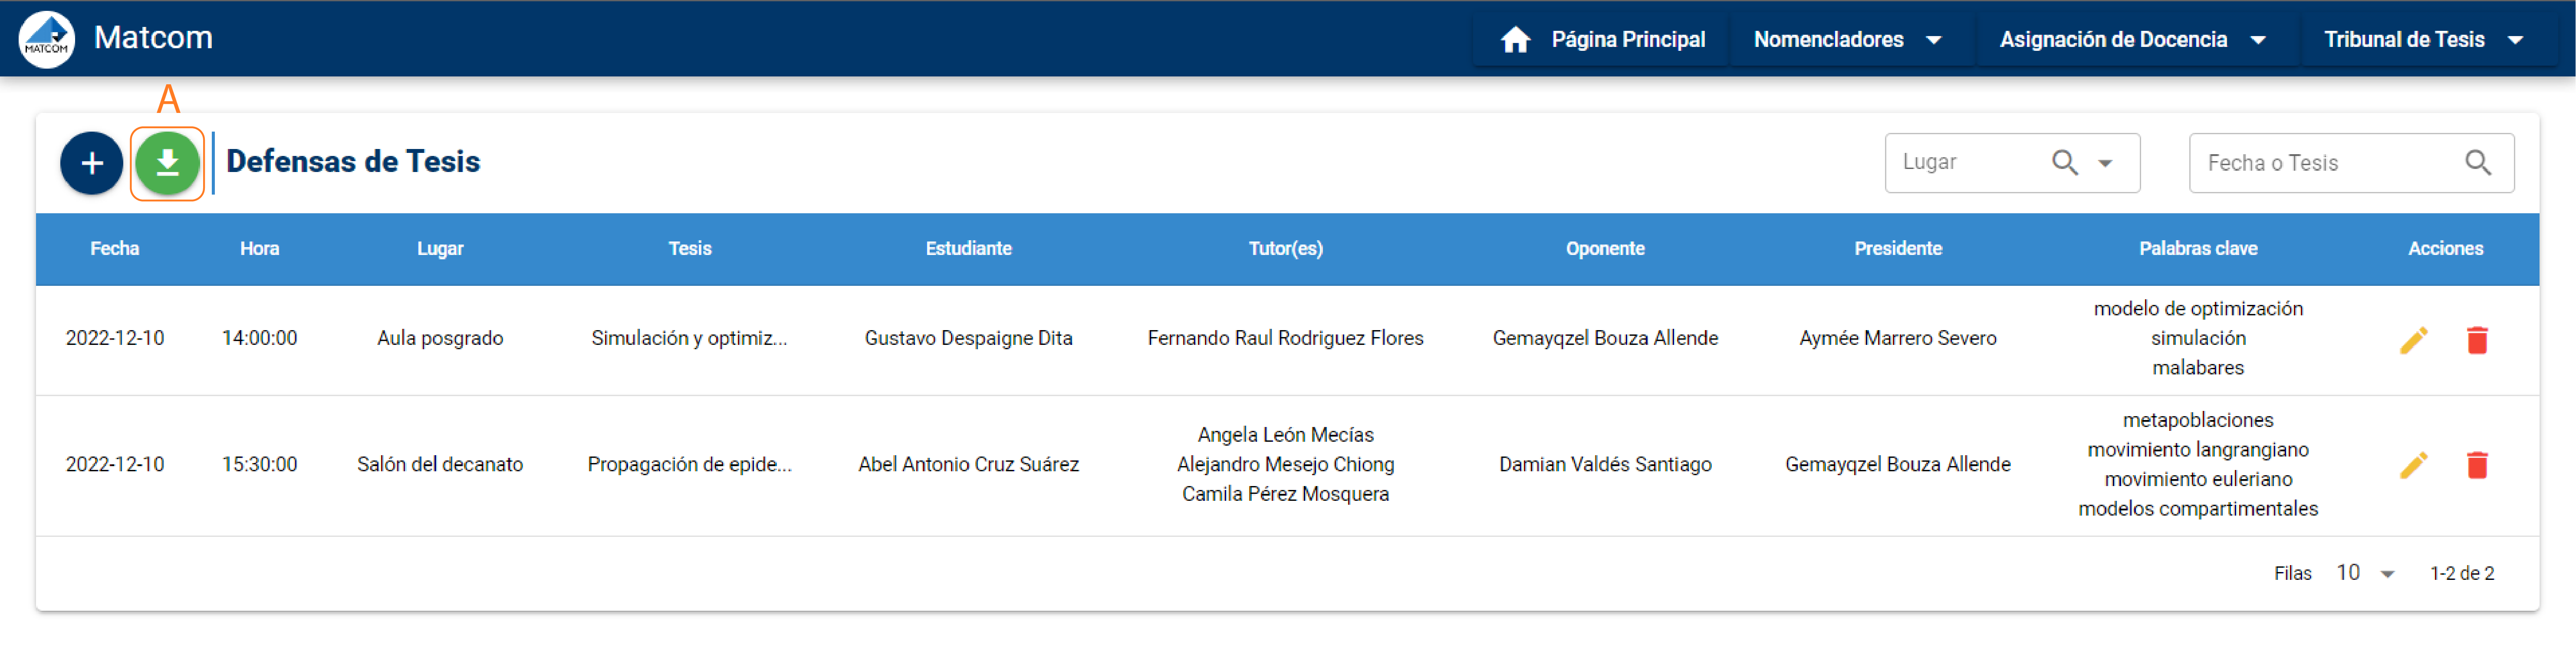
\includegraphics[scale=0.3]{Graphics/Implementation/Tesis/thesis-defense-result.png}
    \caption{Vista resultado de las planificaciones de tesis.}
    \label{img-tc-thesis-defense-result}
\end{figure}

% Para definir la fecha, hora y local donde se realizará la defensa de una tesis, se debe 
% pulsar sobre el botón de editar de la fila correspondiente a la defensa que 
% se desea planificar. En la figura tal se muestra ek resultado de pulsar sobre la fila 
% tal para planificar la defensa de la tesis tal. \\



Para poder llevar a cabo la planificación de las tesis a través
del sistema que se propone, es necesario que en la base de datos 
se ingresen las informaciones que intervienen en este proceso. Por ejemplo 
para poder confeccionar un tribunal es necesario que la tesis haya sido agregada 
anteriormente, pero para poder agregar la tesis es necesario que los tutores y 
cotutores se encuentren en el sistema. Por tanto el primer paso 
para realizar la planificación de las tesis, es ingresar todos los datos que se describen 
en la sección \ref{database:planificación-tesis}


En la siguiente sección se describen otras funcionalidades implementadas 
con el objetivo de agregar utilidad al sistema que se propone.

\section{Exportar e importar datos de la base de datos}\label{cap4:csv}

En el servidor se implementó un módulo 
que permite salvar el estado de la base de datos 
en documentos csv y poblar la base de datos a partir de los mismos.
Se crearon dos comandos para ejecutar en la terminal con el 
fin de realizar las tareas mencionadas previamente:

\subsection{Exportar los datos de la base de datos}

Se implemetó el comando \texttt{save\_database}
que permite exportar una o todas las tablas de la base de datos.
La información de cada tabla se almacena en un archivo CSV.
Para exportar la información de una única tabla
se debe especificar su nombre precedido del argumento \texttt{-m}. Por 
ejemplo para salvar la tabla que contiene la información de los profesores, se debe 
ejecutar el siguiente comando.

\begin{verbatim}
    python manage.py save_database -m Professors
\end{verbatim}


Por otra parte, si lo que se desea es exportar la información de todas las tablas 
de la base de datos a documentos CSV, se debe ejecutar el siguiente comando.

\begin{verbatim}
    python manage.py save_database
\end{verbatim}


\subsection{Importar datos a la base de datos}
Se implementó el comando \texttt{fill\_database} que permite poblar la 
base de datos a partir de los archivos CSV generados con el comando \texttt{save\_database}.
Con este comando se puede poblar una o todas las tablas de la base de 
datos. 
Para poblar la información de una única tabla
se debe especificar su nombre precedido del argumento \texttt{-m}. Por 
ejemplo para llenar la tabla que contiene la información de las asignaturas, se debe 
ejecutar el siguiente comando.

\begin{verbatim}
    python manage.py fill_database -m Subjects
\end{verbatim}

Por otra parte, si lo que se desea es importar la información de todos los archivos CSV  
para la base de datos, se debe ejecutar el siguiente comando.

\begin{verbatim}
    python manage.py fill_database
\end{verbatim}


Los posibles nombres de entidades a utilizar con
el parámetro -m tanto para el comando 
\texttt{save\_database} como \texttt{fill\_database} son:
\texttt{ClassTypes}, \texttt{Faculties},
\texttt{ScientificDegrees}, \texttt{TeachingCategories},
\texttt{Semesters}, \texttt{TeachingGroups}, \texttt{TimePeriods}, \texttt{ScholarYears},
\texttt{Careers}, \texttt{StudyPlans}, \texttt{CarmenTable}, \texttt{Departments},
\texttt{Subjects}, \texttt{Professors}, \texttt{SubjectDescriptions}, \texttt{TeachingAssignments},
\texttt{Places}, \texttt{Keywords}, \texttt{Thesis}, \texttt{ThesisCommittee}. \\


En este capítulo se describieron los pasos a seguir para realizar la asignación de docencia 
y la planificación de las tesis a través del sistema que se propone. Se ilustraron las principales 
funcionalidades que se deseaban incorporar como: conocer la carga docente de los profesores durante 
el proceso de asignación, conocer la cantidad de participaciones de los profesores en los tribunales 
y la exportación de la información de estos procesos a un documento CSV. \\

En el próximo capítulo se describe la estructura del proyecto y algunos 
detalles de implementación que pueden servir para incorporar nuevos procesos 
en el sistema de gestión implementado.

% Se implementó un modelo de optimización para la 
% generación de asignaciones de docencia, pendiente
% computar el peso de las asignaciones (dado las
% preferencias de los profesores y sus habilidades)
